\chapter{Theoretischer Rahmen} \label{chapter:theorie}

In diesem Kapitel wird der theoretische Rahmen für die Arbeit abgesteckt. 
Abschnitt \ref{sec:gram} diskutiert die wichtigsten Modelle und Prinzipien  der \isi{Grammatikalisierung}, die den Wandel von Demonstrativ- zu \isi{Definitartikel} \is{Definitartikel}erfassen. In Abschnitt \ref{sec:kxg} wird dafür argumentiert, den Wandel als einen Fall von \isi{Konstruktionalisierung}, genauer als Herausbildung des Schemas \is{Schema} [Definitartikel\,+\,N] zu begreifen. Abschnitt \ref{sec:mechanismen} diskutiert, inwiefern \isi{Analogie} und \isi{Reanalyse} als zentrale Mechanismen den Wandel vorantreiben.   

\section{Die grammatikalisierungstheoretische Perspektive}\label{sec:gram}

Ein adnominal gebrauchtes \isi{Demonstrativum} ist neben Personal- \is{Personalpronomen} oder Possessivpronomina \is{Possessivum}  die häufigste Quelle für \isi{Definitartikel} \parencites()(){Himmelmann1997}[215]{Heine2002}, so auch für die \isi{Definitartikel} in den indoeuropäischen Sprachen \parencite{vonHeusinger2013}.\footnote{Zu anderen Quellen s. \textcite[839]{Himmelmann2001} oder \textcite[523]{deMulder2011}.}
An Abbildung~\ref{wals} aus dem \textit{World Atlas of Language Structures} (WALS)\footnote{\url{https://wals.info/feature/37A\#2/25.5/148.2}; zuletzt aufgerufen am 19.05.2020.} lassen sich indirekt die groben Stufen der Artikelentwicklung -- vom \isi{Demonstrativum} zu einem affigierten Artikel \is{Affix} -- ablesen. 

\begin{figure}
\begin{center}
  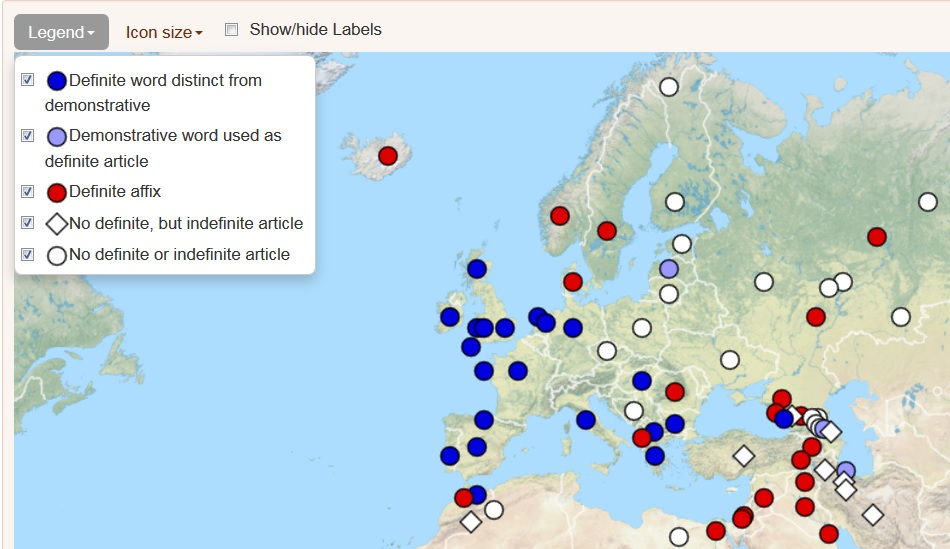
\includegraphics[width=\textwidth]{images/wals.jpg}
\caption {Definitartikel in den Sprachen Europas \parencite{Dryer2013}}
\label{wals}
\end{center}
\end{figure} 

Dargestellt ist die Verteilung von \is{Demonstrativartikel}Demonstrativ-, \is{Definitartikel}Definit- und Indefinitartikeln \is{Indefinitartikel} in den Sprachen Europas: Hellblau markiert sind Sprachen, in denen das \isi{Demonstrativum} Aufgaben eines Definitartikels übernimmt. Dies ist bspw. im westlettischen Dialekt Tahmisch der Fall \parencite[573--574]{Schroeder2006}.
Eine funktionale \isi{Polysemie} wie diese hat in vielen Sprachen dazu geführt, dass sich das \isi{Demonstrativum} formal abspaltet und zum  \isi{Definitartikel} wandelt, so etwa in den (auf der Karte mit einem dunkelblauen Punkt gekennzeichneten) romanischen und westgermanischen Sprachen. Mit zunehmendem Gebrauch kann der \isi{Definitartikel} an lautlicher Substanz 
verlieren \is{Affigierung} und sich zur Flexionsendung \is{Flexion} entwickeln, wie bspw. in den  nordgermanischen Sprachen, vgl. schwed. \object{bok-en} \extrans{das Buch}, die in der Karte mit einem roten Punkt markiert sind.  Die formale Reduktion wird mit einer späten Entwicklungsstufe des Definitartikels gleichgesetzt. Das Verhältnis von Sprachen mit und Sprachen ohne \isi{Definitartikel} hält sich den Daten des WALS zufolge \parencite[Kapitel 37]{Dryer2013} in etwa die Waage (216 zu 198). Ob sich ein \isi{Definitartikel} herausbildet, ist von vielen sprachinternen und -externen Faktoren abhängig. Die slawischen Sprachen verfügen z.B. über keinen Definitartikel, wohl aber über Mittel, Referenten als definit zu kennzeichnen, bspw. mit Hilfe des Verbalaspekts \is{Aspekt} oder durch Kasusoppositionen \is{Kasusopposition} \parencite{Hauenschild1993,Leiss2000}. Sprachen mit einer relativ freien Konstituentenabfolge (z.B. Finnisch oder Chinesisch) nutzen die \isi{Wortstellung}, um definite Referenten syntaktisch zu exponieren.\footnote{Das ursprünglich artikellose Althochdeutsche verfügte über ähnliche Strategien, vgl. Abschnitt \ref{sec:def-ahd}.}

Nachfolgend geht es darum, die hier skizzierten Entwicklungsstufen vor dem Hintergrund grammatikalisierungstheoretischer \is{Grammatikalisierung} Ansätze zu diskutieren und damit den ersten Baustein für das theoretische Fundament der Arbeit zu schaffen. 
In Abschnitt \ref{sec:stufen} werden zunächst die wichtigsten Grammatikalisierungsskalen \is{Grammatikalisierungspfad} beleuchtet.  
Anschließend widmet sich Abschnitt \ref{sec:dem-quelle} dem besonderen Status des Demonstrativums \is{Demonstrativum} als Quelle für den Definitartikel. Abschnitt \ref{sec:parameter} behandelt die für den \isi{Definitartikel} wichtigsten Parameter der \isi{Grammatikalisierung}. 


\subsection{Universelle Entwicklungsstufen}\label{sec:stufen}

In der Forschung wurden einige Modelle vorgeschlagen, die einerseits die Entwicklung vom Demonstrativ- \is{Demonstrativartikel} zum \isi{Definitartikel} erfassen und andererseits die formale und funktionale Weiterentwicklung des Artikels beschreiben. Die prominentesten stammen von \textcite{Greenberg1978} und daran anknüpfend \textcite{Lehmann2015} sowie \textcite{Schmuck2014}. Sie werden an dieser Stelle einführend vorgestellt und mit Blick auf ihre Anwendbarkeit für das Deutsche beleuchtet. Im Vordergrund steht dabei die frühe Phase der Artikelentwicklung. 
%
%\subparagraph*{Greenbergs Definitheitszyklus} 

Greenbergs \hervor{cycle of the definite article} \is{Grammatikalisierungspfad}\is{Definitheit}\parencite[61]{Greenberg1978} umfasst vier Stufen, welche in Abbildung~\ref{abb:greenberg} \parencite[entnommen aus][525]{deMulder2011} wiedergegeben sind.

\begin{figure}
  \begin{tikzpicture}[row 2/.style={font=\scshape}]
  \matrix (greenberg) [inner sep=0pt,matrix of nodes,row sep=.33cm,column sep=\tabcolsep]
    {
      Stage 0 & & Stage I & & Stage II && Stage III\\
      demonstrative & > & definite article & > & specific article & > & noun marker\\
    };
  \draw[-{Triangle[]}] (greenberg.west) -- (greenberg.east);
  \end{tikzpicture}
\caption {Der Definitheitszyklus \is{Grammatikalisierungspfad}\is{Definitheit}nach \textcite{Greenberg1978}\label{abb:greenberg}}
\end{figure}

Die Skala korreliert mit einem Abbau der \isi{Referentialität}: Aus einem \isi{anaphorisch} gebrauchten \isi{Demonstrativum} (Stage 0) wird ein Definitartikel, der dazu beiträgt, Referenten als identifizierbar zu kennzeichnen (Stage I). In der nächsten Stufe erfolgt die Ausweitung auf spezifische, \is{Spezifizität} aber nicht identifizierbare Referenten (Stage II), so dass der \isi{Definitartikel} in das Arbeitsfeld der Indefinita \is{Indefinitartikel} eindringt. Am Ende spielt die \isi{Referentialität} keine Rolle mehr: Der Artikel fungiert entweder als bloßer Genusmarker \is{Genus} oder -- und dies ist der Fall, wenn das ursprüngliche \isi{Demonstrativum} das Nomen nicht nach \isi{Genus} klassifiziert hat -- als Marker der \isi{Nominalität} \parencite[Stage III;][69]{Greenberg1978}. In dieser Rolle hilft er bspw., deverbale Nomen zu kennzeichnen. Die Entwicklung wird in der Regel begleitet von einem graduellen phonetischen Schwund, was Affigierungsprozesse \is{Affigierung} nach sich ziehen kann und der Zyklus von Neuem beginnt. In vielen germanischen Sprachen erfährt das ursprüngliche \isi{Demonstrativum} bereits eine erneute formale Stärkung \parencite[302--303]{vanGelderen2007}. Häufig wird die deiktische Komponente mit Hilfe von Lokaladverbien \is{Adverb} neu aufgebaut \parencite[s.][]{Diessel1999}, so auch im Deutschen (etwa:  \object{der da, das hier}). 

Bemerkenswerterweise ist der Zyklus nicht das Resultat von Überlegungen, wie Demonstrativa \is{Demonstrativum} zu Definitartikeln als Marker von \isi{Definitheit} werden, sondern wie sich \isi{Definitartikel} zu Genusmarkern \is{Genus} entwickeln. Entsprechend steht der emergierende Artikel nach Greenberg vornehmlich im Dienste einer eindeutigen und regelmäßigen Genusmarkierung \is{Genus} am Nomen, welche von Affixen \is{Affix} am Nomen nicht mehr gewährleistet wird, so etwa in den Niger-Kongo-Sprachen \parencite[55, 62]{Greenberg1978}. Dass diese Erklärung zum Ursprung des Definitartikels nicht für alle Sprachen greift, haben zahlreiche Studien herausgestellt, welche den Übergang als komplexe Verschiebung innerhalb der Domäne der \isi{Definitheit} beschreiben \parencite[z.B.][]{Himmelmann1997,Lyons1999,Leiss2000,Demske2001}, vgl. hierzu ausführlich Abschnitt \ref{sec:gruende}.

Auch die grobe lineare Dreischrittigkeit \isi{Demonstrativum} -- \isi{Definitartikel} -- Spezifizierer \is{Spezifizität} ist nicht unproblematisch. Denn erstens verläuft in vielen Sprachen (so auch im Deutschen) die \isi{Spezifizität} orthogonal zur \isi{Definitheit}, s. die Beispiele in \REF{ex:spez-ortho} in Adaption an \textcite[245]{Studler2011}; vgl. auch \textcite{Lyons1999}. 

\begin{exe}
\settowidth\jamwidth{(spez./def.)}
	\ex \label{ex:spez-ortho}   
	\begin{xlist}
		\ex \label{ex:kleid1} Er sucht einen Übersetzer.  \jambox{(unspez./indef.)} 
		\ex \label{ex:kleid2} Sie hat gestern ein Auto gekauft. \jambox{(spez./indef.)}
		\ex \label{ex:stud1} Der erste Anrufer bekommt einen Preis. \jambox{(unspez./def.)}
		\ex \label{ex:stud2} Der Nachtisch gestern war sehr gut. \jambox{(spez./def.)}
		\end{xlist}
\end{exe}

\noindent 
Zweitens müssen anscheinend nicht alle Stadien zwangsläufig durchlaufen werden: \textcite[107]{Himmelmann1997} und \textcite[139]{Diessel1999} merken z.B. an, dass nicht nur Definitartikel, sondern auch Demonstrativa \is{Demonstrativum} als spezifische \is{Spezifizität} Artikel fungieren können, vgl. das Beispiel in \REF{ex:guy} aus \textcite[533]{deMulder2011}. 
\begin{exe}
	\ex \label{ex:guy}   There was this guy in my class last quarter.
\end{exe}
\noindent 
Anders als im Deutschen schwingt hier keine pejorative Lesart mit, sondern die Phrase \object{this guy} dient zur Einführung eines neuen und für den späteren Diskurs wichtigen Referenten. In diesem Fall wurde Stage I also übersprungen. 

Zudem müsste die letzte Entwicklungsstufe (Stage III) weiter ausdifferenziert werden. So kann der deutsche \isi{Definitartikel} gegenwärtig zwar als nominaler Marker \is{Nominalität}betrachtet werden -- etwa wenn er Eigennamen \is{Eigenname} begleitet (\object{die Pia}) oder Substantivierungen \is{Substantivierung} (\object{das Laufen}) kenntlich macht \parencite[71]{Szczepaniak2011a}. Andererseits zeigt er auch Tendenzen, sich zu einem \object{classifier} zu entwickeln, indem er u.a. ontologische (\object{die Bismarck} = Schiffsname) oder sozio-pragmatische Klassifikationen (z.B. denunziatorisch: \object{die Merkel}) über unterschiedliche Genera \is{Genus} abbildet \parencite{Nubling2014}. Greenberg selbst merkt an, dass Phasen parallel verlaufen können und es sich um einen graduellen Prozess mit möglichen Ausnahmen handelt \parencite[61]{Greenberg1978}. Nur über empirische Forschungen, idealerweise mit Blick auf diachrone Etappen von einzelnen Sprachen, kann dieser Prozess hinreichend beschrieben werden. 

Im Gegensatz zu Greenbergs Modell, das die Frühphase der Artikelentwicklung kaum thematisiert, setzt die darauf aufbauende Skala \is{Grammatikalisierungspfad} von \textcite{Lehmann2015} eine Stufe zwischen  Demonstrativ- \is{Demonstrativartikel} und \isi{Definitartikel} an und eröffnet damit Raum für Diskussionen, wie der kategoriale Wandel ablaufen könnte. Lehmann selbst kommentiert diesen Aspekt allerdings nur relativ kurz, indem er anmerkt:\hervor{[T]he demonstrative component is gradually reduced to mere definiteness, and the result is a definite article} \parencite[41]{Lehmann2015}. Sein Modell ist in Abbildung~\ref{abb:lehmann} wiedergegeben. 

\begin{figure}
\smartdiagramset{border color=black,
set color list={white,white,white,white,white},
uniform arrow color=true,
arrow color=black,
back arrow disabled=true}
\resizebox{\textwidth}{!}{\smartdiagram[flow diagram:horizontal]{demonstrative determiner, weakly demonstrative definite determiner, definite article, affixal article, noun marker}}
\caption {Der \isi{Grammatikalisierungspfad} von \textcite[59]{Lehmann2015}\label{abb:lehmann}}
\end{figure}

Aus Lehmanns Sicht bildet der anaphorische \is{anaphorisch} \isi{Demonstrativartikel} den Ausgangspunkt für die Entwicklung des Definitartikels \parencite[ebenso:][]{Greenberg1978,Lyons1999}. Seit der Monographie von \textcite{Himmelmann1997} wird auch der anamnestische Gebrauch \is{anamnestisch} als \hervor{Sprungbrett} für die \isi{Grammatikalisierung} \parencite[74]{Szczepaniak2011a} betrachtet \parencite[s. hierzu auch den Überblick in][527]{deMulder2011}. Für viele Sprachen fehlen jedoch Studien, die diese Entwicklungsstufe empirisch dokumentieren und mögliche  Brückenkontexte \is{Brückenkontext} \parencite[84]{Heine2002a} offenlegen, so auch für das Deutsche. Eine ausführliche  Auseinandersetzung mit diesem Aspekt erfolgt in Abschnitt \ref{sec:bruecke} der vorliegenden Arbeit.

Kritisch an Lehmanns \isi{Grammatikalisierungspfad} ist die Vermischung von formalen und funktionalen Aspekten des Wandels. Seine Skala suggeriert nämlich, dass die Stufe des affigierten \is{Affix} Artikels eine diskrete, eigenständige Phase ist. Der Verlust an phonetischer Substanz ist jedoch ein Beiprodukt, das -- abhängig von den typologischen Eigenheiten einer Sprache \parencite[vgl.][33]{Himmelmann2004} -- mit jeder Entwicklungsstufe einhergehen kann. Beispielsweise treten schon im  Althochdeutschen Präpositionen-Artikel-Klisen \is{Klitikon} auf, etwa \object{zi themo} > \object{zemo} \extrans{zu dem} \parencite{Schlachter2015}, also zu einer Zeit, in der der \isi{Definitartikel} erst am Anfang der \isi{Grammatikalisierung} steht. Bis heute liegt hier eine \hervor{Grammatikalisierungsbaustelle}   \parencite{Nubling1992,Nubling2005} vor, da die Verschmelzung u.a. durch phonologische und semantische Faktoren blockiert wird \parencite[s. auch][91]{Szczepaniak2011a}.
Entscheidend für den kategorialen Übergang von Demonstrativ- \is{Demonstrativartikel} zu \isi{Definitartikel} ist also die funktionale Seite des Wandels. \textcite{Schmuck2014} schlagen mit der Skala in Abbildung~\ref{abb:schmuckszczep} \parencite[aufbauend auf][]{Lyons1999,Szczepaniak2011a} einen \isi{Grammatikalisierungspfad} vor, der die funktionale Seite des Wandels in Bezug auf das ahd. \object{dër} \extrans{dieser} beschreibt. 

\begin{sidewaysfigure}
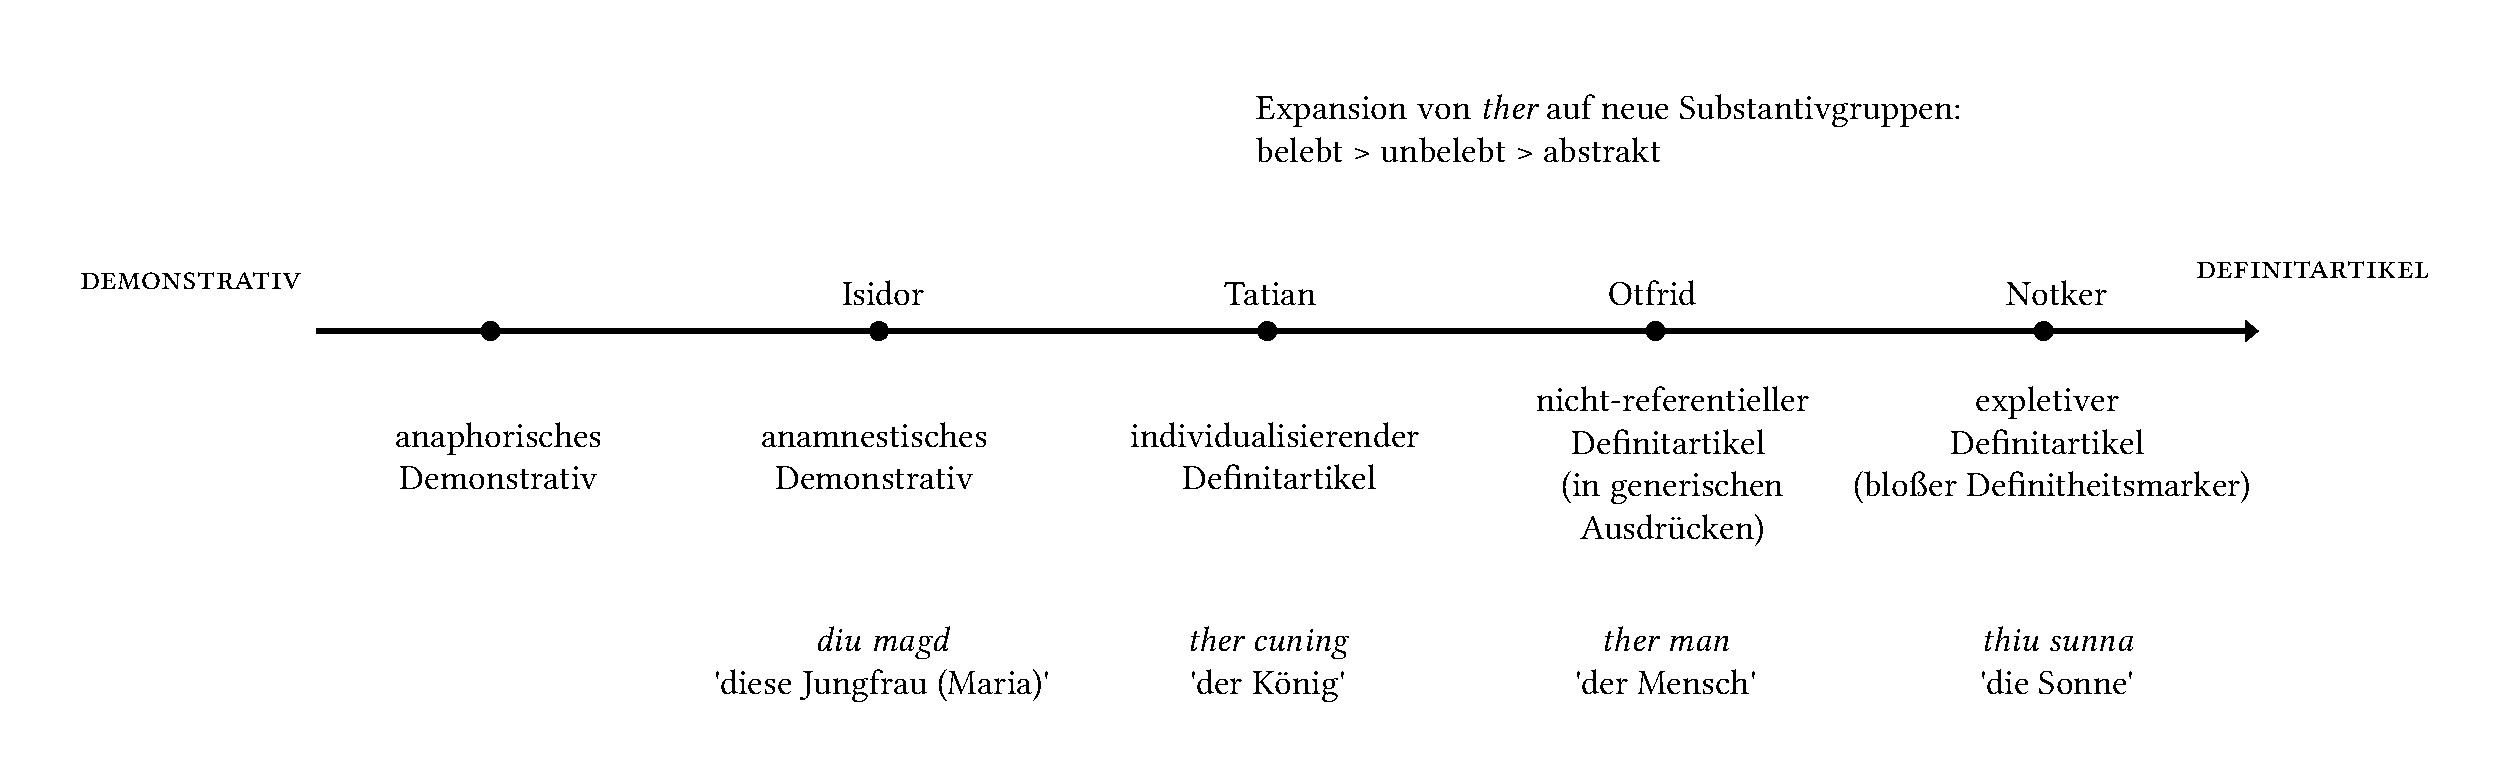
\includegraphics[width=\textwidth]{images/schmuckszczep.pdf}
\caption {Die \isi{Grammatikalisierung} des Definitartikels im Ahd. \parencite[102]{Schmuck2014}\label{abb:schmuckszczep}}
\end{sidewaysfigure}
 
Die Skala bildet die folgenden Entwicklungsstufen ab \parencite[vgl. auch][69--78]{Szczepaniak2011a}: Im frühen Althochdeutschen (repräsentiert durch Isidor, der um 780 entstanden ist), wird das \isi{Demonstrativum} vornehmlich gebraucht, um einen Referenten mittels Diskursinformationen (anaphorischer Gebrauch) \is{anaphorisch} oder mit Bezug auf gemeinsames Vorwissen (anamnestischer Gebrauch) \is{anamnestisch}\is{Definitheitskontext}von anderen potentiellen Referenten abzugrenzen. Das Herstellen solcher kontextabhängigen Bezüge ist charakteristisch für Demonstrativa \is{Demonstrativum} \parencite[85]{Himmelmann1997}. Im Laufe der Zeit verliert das Artikelwort  seine demonstrative Komponente und es wird möglich, auch ohne Kontext die eindeutige Referenz zu markieren (individualisierender Gebrauch). Damit ist der Weg für Gebrauchskontexte geebnet, die ausschließlich Definitartikeln vorbehalten sind, darunter nicht-referentielle (generische) Gebrauchskontexte \is{generisch} sowie die Kombination mit Unika \is{Unikum} (expletiver Artikel), \is{Expletiver Artikel} die \textcite{Oubouzar1989,Oubouzar1992} schon bei Otfrid (um 870) und regelmäßiger bei Notker (um 1025) beobachtet. Die nächste Entwicklungsstufe ist die Ausweitung auf den onymischen Wortschatz, \is{Eigenname} die allerdings erst im Frühneuhochdeutschen (Frnhd.) einsetzt \parencite[s. ausführlich][]{Schmuck2014}. 

Ein zentrales Ziel der vorliegenden Arbeit ist es, die hier skizzierten Definitheitskontexte, \is{Definitheitskontext} welche in Kapitel \ref{chap:demdef} noch ausführlich beschrieben werden, mithilfe einer computergestützten Korpusanalyse in Bezug auf das ahd. \object{dër} zu untersuchen. Das Modell von \textcite{Schmuck2014} fungiert als theoretischer Ausgangspunkt und wird in Kapitel \ref{bicpic} auf Basis der gewonnenen Ergebnisse modifiziert. Wie man in Abbildung~\ref{abb:schmuckszczep} sieht, gehen \textcite{Schmuck2014} davon aus, dass die \isi{Expansion} des Definitartikels belebtheitsgesteuert \is{Belebtheit} (belebt > unbelebt > abstrakt) verläuft. Diese Hypothese wird auch in der vorliegenden Arbeit aufgenommen. Kapitel \ref{chapter:belebtheit} erläutert die Verbindung von Belebtheit \is{Belebtheit} und Artikelsetzung ausführlich. 

 
\subsection{Primäre oder sekundäre Grammatikalisierung?} \label{sec:dem-quelle}

Am Anfang von Grammatikalisierungsprozessen \is{Grammatikalisierung} stehen typischerweise lexikalische Elemente \is{Morphem} \parencite[s. ausführlich][]{Heine1991,Hopper1991,Traugott1991,Bybee1994,Lehmann2015}:  \blockcquote[4]{Bybee1994}{Reduced to its essentials, grammaticalization theory begins with the observation that grammatical morphemes develop gradually out of lexical morphemes or combinations of lexical morphemes with lexical or grammatical morphemes}. 
Ein klassisches Grammatikalisierungsbeispiel ist die Entwicklung von Vollverben zu Hilfsverben: So entwickelt sich das \object{going-to}-Futur z.B aus dem Vollverb \object{gehen} \parencite[s.][70--71]{Heine1991}. Der funktionale Shift wird meist von formalen Reduktionsprozessen \is{Klitikon} begleitet (\object{going to} > \object{gonna}) und führt durch die graduelle semantische Ausbleichung \parencite{Heine2003} zur steten Kontextausweitung \parencite{Himmelmann2004}.  

Mit Blick auf den Ursprung handelt es sich also beim Wandel vom Demon"-stra"-tiv- zum \is{Demonstrativartikel} \isi{Definitartikel} um einen speziellen Grammatikalisierungsprozess. Vereinfacht gesprochen entwickelt sich aus einem bereits vorhandenen grammatischen Element (dem Demonstrativartikel) eine neue grammatische Form. Dieser Prozess wird daher auch \object{sekundäre} \isi{Grammatikalisierung} \parencite{Givon1991, Detges2002, Szczepaniak2011a} genannt -- im Kontrast zu \object{primären} Grammatikalisierungen, an deren Beginn lexikalische Elemente stehen \parencite[81]{Traugott2002}.
Es ist allerdings fraglich, ob die sekundäre \isi{Grammatikalisierung} als eigene Entwicklungsstufe betrachtet werden sollte, die zeitlich auf eine frühere \isi{Grammatikalisierung} folgt. Für Givón, der den Terminus Anfang der 1990er in den Forschungsdiskurs einführt, ist eine solche Chronologie definitorisch: \blockcquote[][193]{Givon1991}{What is suggested in this article is that exis"-ting, earlier-grammaticalized morpho-syntax can give rise, via secondary grammaticalization, to other mor\-pho-syn\-tac\-tic patterns}.

In Bezug auf die \isi{Grammatikalisierung} des Definitartikels \is{Definitartikel} lassen sich einige Argumente gegen die Annahme anführen, dass es eine lexikalische Quelle für das \isi{Demonstrativum} gibt und damit eine primäre \isi{Grammatikalisierung} der Entwicklung des Definitartikels vorausgeht: Laut \textcite[150]{Diessel1999} wurde bislang für keine Sprache der empirische Nachweis erbracht, dass Demonstrativa \is{Demonstrativum} von lexikalischen Elementen abstammen (die o.g. Strategien zur Stärkung der deiktischen Komponenten ausgenommen). Dennoch verfügen alle Sprachen über Demonstrativa \is{Demonstrativum} \parencite[1]{Diessel1999}. Neben Inhaltswörtern wie \object{Mama} oder \object{Ball} zählen demonstrative Ausdrücke zum frühen Wortschatz von Kindern; oft gehören sie zu den ersten zehn Wörtern, die erlernt werden \parencite[476]{Diessel2006}. Beides spricht dafür, Demonstrativa \is{Demonstrativum} zum linguistischen Grundinventar zu zählen. Auch funktional nehmen Demonstrativa \is{Demonstrativum} eine Sonderrolle ein: Während typische grammatische Elemente (z.B. Präpositionen) innersprachliche Relationen zwischen Lexemen anzeigen (z.B. \object{auf/unter/über dem Tisch}), liegt die Funktion von Demonstrativa \is{Demonstrativum} darin, die Aufmerksamkeit von Adressaten auf bestimmte Objekte in der außersprachlichen Umgebung zu lenken \parencites{Diessel2006}. 
%[152]{Diessel1999}
Auch innersprachlich sind Demonstrativa \is{Demonstrativum} zentrale diskursstrukturierende Element: Mit ihnen werden prominente Referenten anaphorisch \is{anaphorisch} wiederaufgenommen oder Topikwechsel \is{Topik} eingeleitet. Wie in Abschnitt \ref{sec:kata} noch gezeigt wird, ist es gerade diese kommunikative Zeigefunktion, welche die \isi{Grammatikalisierung} überhaupt erst ankurbelt: Sprecherinnen und Sprecher nutzen sie aus, um wichtige, d.h. in erster Linie belebte und agentive Referenten \is{Belebtheit}\is{Agentivität}zu exponieren. Der inflationäre Gebrauch führt dazu, dass sich die Zeigefunktion langsam abnutzt und auch Referenten, die auf der Belebtheitsskala \is{Belebtheitshierarchie} hierarchisch niedriger angesiedelt sind, regelmäßig mit dem emergierenden Artikel \is{Definitartikel}determiniert werden (vgl. hierzu ausführlich Kapitel~\ref{chapter:belebtheit}).


\textcite{Breban2014} argumentiert plausibel dafür, dass eine Zweiteilung in primäre und sekundäre \isi{Grammatikalisierung} schließlich keinen definitorischen Mehrwert liefert.
Stattdessen plädiert sie für eine breitere Auslegung von Grammatikalisierung, die auch grammatische Elemente als mögliche Quelle für den Wandel in Betracht zieht und damit die Artikelentwicklung als \isi{Grammatikalisierung} einschließt  \parencite[zur weiterführenden Diskussion s.][]{Breban2012}: \blockcquote[498]{Breban2014}{[G]rammaticalization processes can have lexical, grammatical, or grammaticalized items/constructions as input. Whatever the nature of the input, the subprocesses of changes involved appear to be the same. [...] [G]ramma\-ticalization processes consist of a complex of changes that affect different domains of change, and happen at different stages in the grammaticalization process.}

\noindent 
Um die Charakteristika des Wandels und die im Zitat genannten \object{domains of change} zu erfassen, wurden in der Grammatikalisierungsforschung unterschiedliche Parameter \is{Grammatikalisierungsparameter} vorgeschlagen, die nachfolgend mit Blick auf die Entwicklung des Definitartikels diskutiert werden.   


\subsection{Parameter der Grammatikalisierung}\label{sec:parameter}

Nach \textcite[96--112]{Traugott2013} lassen sich zwei Hauptzweige in der Grammatikalisierungsforschung unterscheiden. Zum einen existiert ein großes und traditionsreiches Forschungsfeld \parencite[hierzu zählen u.a. die Arbeiten von][]{Givon1979,Haspelmath2004,Lehmann2015,}, in dem \isi{Grammatikalisierung} vor allem als gradueller Autonomieverlust des betroffenen sprachlichen Zeichens betrachtet wird, begleitet von formalen Reduktionsprozessen. Der andere Forschungszweig begreift \isi{Grammatikalisierung} als Prozess der Kontextexpansion \is{Expansion} \parencite{Himmelmann1997,Himmelmann2004}. 

Die Lehmannschen Grammatikalisierungsparameter \is{Grammatikalisierungsparameter} sind für die erste genannte  Forschungsrichtung exemplarisch, s. Tabelle~\ref{tab:lehmann-parameter-prozess}, entnommen aus \textcite{Lehmann1995}. Mit ihnen kann man sprachliche Zeichen hinsichtlich ihres Grammatikalisierungsgrades auf syntagmatischer und paradigmatischer Ebene vergleichen. 

%
\begin{table}
\centering
\small
\begin{tabular}{
	l
	>{\raggedright}p{2,75cm}
	c
	>{\raggedright\arraybackslash}p{2,75cm}
}
\lsptoprule
& \multicolumn{3}{c}{{Grammatikalisierungsgrad}}\\
                   & \multicolumn{1}{c}{{niedrig}}& & \multicolumn{1}{c}{{hoch}}\\
\cmidrule(lr){2-4}
{Parameter} & & {Prozess}   &                   \\ \midrule
{Paradigmatizität}            & Zeichen gehört zu losem Wortfeld                         & Paradigmatisierung & Zeichen gehört zu hochintegriertem Paradigma                     \\
{Wählbarkeit}                 & Zeichen ist nach kommunikativen Absichten frei wählbar   & Obligatorisierung  & Wahl des Zeichens ist beschränkt bzw. obligatorisch              \\
{Integrität}                  & Bündel semantischer Merkmale; evtl. mehrsilbig           & Erosion            & grammatische Merkmale; oligo- oder monosegmental                 \\
{Fügungsenge}                 & Zeichen ist unabhängig juxtaponiert                      & Koaleszenz         & Zeichen ist \isi{Affix} oder bloß phonologische Eigenschaft des Trägers \\
{Stellungsfreiheit}           & Zeichen ist frei umstellbar                              & Fixierung          & Zeichen besetzt feste Position                                   \\
{Skopus}                      & Zeichen bezieht sich auf Syntagma beliebiger Komplexität & Kondensierung      & Zeichen modifiziert Stamm                                        \\ \lspbottomrule
\end{tabular}
\caption{Parameter und Prozesse der \isi{Grammatikalisierung} \parencite[1255]{Lehmann1995}}
\label{tab:lehmann-parameter-prozess}
\end{table}

 
Der \isi{Definitartikel} zeigt im Gegenwartsdeutschen gemäß dieser Parameter \is{Grammatikalisierungsparameter} einen im Vergleich zu seinem demonstrativen Vorläufer erhöhten Grammatikalisierungsgrad. \is{Grammatikalisierung}

\begin{description}
\item[Paradigmatizität:]\sloppy Der \isi{Definitartikel} bildet in Opposition zum \isi{Indefinitartikel} eine geschlossene grammatische Klasse, die im Ahd. nicht gegeben ist. Das Zahlwort \object{eins} entwickelt sich erst im Laufe des Mittelhochdeutschen (Mhd.) zum \isi{Indefinitartikel} \parencite{Szczepaniak2016}. 
\item[Wählbarkeit:] Im Ahd. konnte der \isi{Demonstrativartikel} relativ frei nach dem kommunikativen Ermessen der Sprecherinnen und Sprecher gesetzt werden \parencite{Oubouzar1992}. Im Gegenwartsdeutschen ist die Determinierung des Nomens mit Artikelwort die Regel. 
\item[Integrität:] Durch seine ursprünglich deiktischen und demonstrativen Komponenten vereint der \isi{Demonstrativartikel} mehr semantische Merkmale als der heutige Definitartikel, dessen Bedeutung abstrakter ist und -- vereinfacht gesagt-- auf \isi{Definitheit} reduziert wurde \parencite[41]{Lehmann2015}.
\item[Fügungsenge:] Unauflösbare Präpositionen-Artikel-Enklisen (z.B. \object{im, am}) \is{Klitikon} im Gegenwartsdeutschen zeigen, dass der Artikel an Autonomie eingebüßt hat und damit das Potential besitzt, sich zu einem Flexionsaffix \is{Affix} weiterzuentwickeln \parencite[s. hierzu][]{Nubling1992,Nubling2005}.  
\item[Stellungsfreiheit:] Der \isi{Demonstrativartikel} kommt im Ahd. sowohl prä- als auch postnominal vor \parencite[27--28]{Schrodt2004} und ist damit syntaktisch unabhängiger als der gegenwärtige \isi{Definitartikel}, dessen Stellung vor dem nominalen Kern fixiert ist. \is{Wortstellung}
\item[Skopus:] Als Substantivmarker (z.B. \object{das Lernen}) beschränkt sich der \isi{Skopus} des Definitartikels nur noch auf Wortebene \parencite[71]{Szczepaniak2011a}. In klitisierter Form \is{Klitikon} kann der Artikel nicht über restriktive Nebensätze operieren: \object{Sie geht ?zum/zu dem Zahnarzt, der ihr empfohlen wurde} \parencite[112]{Nubling2005}.
\end{description}

\noindent
Neben der Stellungsfreiheit \is{Wortstellung} und der Integrität ist für die Untersuchung des ahd. Demonstrativums \is{Demonstrativum} die Wählbarkeit der wohl wichtigste Aspekt. Denn wenn das Artikelwort nicht mehr variabel, sondern obligatorisch gesetzt wird, bildet es zusammen mit dem Bezugsnomen eine feste Einheit zum Ausdruck definiter Referenz \is{Definitheit} [\object{dër}\,+\,N] (s. Abschnitt \ref{sec:konstruktionalisierung}). 

Lehmanns strukturalistisch angelegte Parameter \is{Grammatikalisierungsparameter} prägen ein Grammatikalisierungsbild, das den Autonomieverlust eines einzelnen sprachlichen Zeichens in den Vordergrund stellt. Pragmatische Aspekte des Wandels und insbesondere metaphorische \is{Metapher} und metonymische \is{Metonymie} Kommunikationsstrategien, die Grammatikalisierungen \is{Grammatikalisierung} vorantreiben, werden dabei wenig beachtet. Dabei zeigen z.B. \textcite[84--93]{Hopper2006}, dass metonymische \is{Metonymie} Prozesse für kontext-indizierte Implikaturen sorgen, die bspw. die Entwicklung des \object{going-to}-Futurs bewirken. Die analogische Ausbreitung \is{Analogie} verläuft in diesem Fall entlang der metaphorischen \is{Metapher} Abstraktion \textsc{Raum > Zeit}\footnote{Die Kapitälchen kennzeichnen \blockcquote[85]{Hopper2006}{abstract, cross linguistic meanings, as opposed to language specific lexical items}.} \parencite[s. auch][45--46]{Heine1991}. Abschnitt \ref{sec:mechanismen} liefert eine ausführliche Diskussion der Rolle von \isi{Analogie} und \isi{Reanalyse} in Bezug auf den Definitartikel. 

Ein weiteres wichtiges Prinzip der Grammatikalisierung, das \citeauthor{Lehmann1995}s Modell nicht direkt abbildet, ist die Tatsache, dass ein Sprachzeichen durch die graduelle semantische Ausbleichung  (in \citeauthor{Lehmann1995}s  Terminologie die \object{Erosion}) im Laufe der Zeit ein immer größeres Spektrum an Gebrauchskontexten abdecken kann und frühere Restriktionen ablegt. Dies lässt sich ebenfalls am \object{going-to}-Futur illustrieren: Während ursprünglich  nur bewegungsfähige Subjekte \is{Subjekt} möglich waren (etwa: \object{I am going to the store}), können heute auch unbelebte Referenten \is{Belebtheit} in der Subjekts"-position vorkommen \is{Subjekt} \parencite[etwa: \object{The tree is going to lose its leaves}; Beispiele nach][5--6]{Bybee1994}. 

\textcite{Himmelmann1997,Himmelmann2004} entwickelt vor diesem Hintergrund ein Sprachwandelkonzept, in dem \isi{Grammatikalisierung} als "`process of context-expansion"'\linebreak \parencite[32]{Himmelmann2004} \is{Expansion}verstanden wird. Damit gilt er als einer der Hauptvertreter des zweiten grammatikalisierungstheoretischen Zweigs, den \textcite[105--109]{Traugott2013} in ihrer Übersicht anführen. Nach \citeauthor{Himmelmann2004} gibt es drei Arten der Kontextexpansion, die \is{Expansion} \object{host-class expansion}, die \object{syntactic context expansion} und die \object{semantic-pragmatic context expansion}, die er am Beispiel des Definitartikels erläutert \parencite[s.][32--33]{Himmelmann2004}: 

\begin{description}
\item[Host-class expansion:] Lockerung der Kollokationsbeschränkungen und damit\linebreak steigende Kombinierbarkeit des grammatikalisierenden Elementes auf syntagmatischer Ebene: Der \isi{Definitartikel} erscheint mit immer mehr Substantivklassen. Dadurch wird u.a. die schrittweise Kombination mit Unika \is{Unikum} oder Eigennamen \is{Eigenname} möglich, welche das ursprüngliche \isi{Demonstrativum} nicht leisten kann. 
\item[Syntactic context expansion:] Anstieg \is{Expansion} der größeren syntaktischen Kontexte, in denen der grammatikalisierende Ausdruck erscheint: Der emergierende \isi{Definitartikel} ist \textcite[32]{Himmelmann2004} zufolge zunächst auf die Subjekts- \is{Subjekt}und Objektsposition  \is{Objekt}beschränkt und kann dann in weniger zentrale Argumentpositionen (z.B. Adverbiale) \is{Adverbial}expandieren \is{Expansion}\parencite[s. hierzu auch ausführlich][]{Himmelmann1998}. 
\item[Semantic-pragmatic context expansion:] Anstieg \is{Expansion}der Gebrauchskontexte, in de-\linebreak nen der Ausdruck gewählt wird: Beim emergierenden \isi{Definitartikel} kommen zu den ursprünglichen pragmatisch-definiten (situationsabhängigen) Gebrauchskontexten semantisch-definite (situationsunabhängige) Ge-\linebreak brauchskontexte hinzu. \is{Pragmatische Definita}\is{Semantische Definita}\is{Definitheitskontext}

 
\end{description}

\noindent
Die Expansionstypen \is{Expansion}bedingen sich gegenseitig: Der Abbau von semantischen Merkmalen (und der gleichzeitige Aufbau neuer grammatischer Funktionen)\linebreak führt dazu, dass ein Zeichen in immer neuen syntaktischen Kontexten verwendet werden kann. Umgekehrt hat jeder Gebrauch in neuen Kontexten zur Folge, dass sich die neue Funktion etabliert. Die graduelle Obligatorisierung der Form und die damit zusammenhängenden Reduktionsprozesse, die Lehmanns Modell hervorhebt, sind nach \textcite[33]{Himmelmann2004} lediglich Epiphänome des Wandels. Während die \herkur{host class expansion} \is{Expansion}von der \isi{Belebtheit}  beeinflusst wird (s. Abschnitt~\ref{sec:belebtwandel}), kommen bei der \herkur{syntactic context expansion} \is{Expansion}die semantische Rolle \is{Semantische Rolle} und damit zusammenhängend die \isi{Referentialität} als Faktoren ins Spiel (s. Abschnitt \ref{sec:partizipanten}).

Durch die bisherigen Ausführungen wurde bereits implizit deutlich, dass\linebreak Sprachzeichen nur innerhalb bestimmter syntagmatischer Kontexte grammatikalisieren.\footnote{Eine Zusammenfassung der Grammatikalisierungsansätze, die explizit den Kontext hervorheben, bietet \textcite{Traugott2003,Traugott2008a}.} 
Diese Erkenntnis ist zwar nicht neu, sie führt aber zu einer wichtigen systemlinguistischen Präzisierung, welche Himmelmann in Bezug auf den \isi{Definitartikel} wie folgt darlegt: \blockcquote[31]{Himmelmann1997}{In Grammatikalisierungsprozessen \is{Grammatikalisierung} wird nicht nur ein Element, das Grammem, sondern ein Ausdrucksmuster (eine Konstruktion) grammatikalisiert. Folglich stellt die Formulierung \extrans{ein \isi{Demonstrativum} entwickelt sich zu einem Definitartikel} \is{Definitartikel}eine Verkürzung dar. Präziser formuliert besteht der Prozeß darin, daß das Ausdrucksmuster Nomen\,+\,Deiktikon sich zu einem Ausdrucksmuster Nomen\,+\,grammatikalisiertes D-Element\footnote{Mit \object{D-Elementen} sind adnominal gebrauchte Lokaldeiktika gemeint \parencite[6]{Himmelmann1997}.} 
 entwickelt.} 
Was Himmelmann vortheoretisch als \object{Konstruktion} \is{Konstruktion}bezeichnet, ist in kon\-struk\-tions\-grammatischen Ansätzen die zentrale Einheit von Sprachen \parencite[s. u.a.][]{Goldberg1995,Goldberg2006}. Daher erscheint es rückblickend fast als logische Konsequenz, dass die historische Sprachwissenschaft die \isi{Konstruktionsgrammatik} für die\linebreak Sprach"-wandel"-for"-schung rekrutiert hat. Das Ergebnis ist die \object{diachrone Konstruktionsgrammatik} \parencite[vgl. u.a.][]{Barddal2015}, innerhalb derer die gängigen Grammatikalisierungstheorien maßgeblich weiterentwickelt wurden (s. hierzu u.a.\citealt{Traugott2003,Bergs2008,Diewald2008,Fried2013,Traugott2013}). Die vorliegende Untersuchung knüpft an diese Forschung an, indem die Entwicklung des Definitartikels als \object{\isi{Konstruktionalisierung}} betrachtet wird -- ein Prozess, der nachfolgend im Rahmen des hier verwendeten konstruktionsgrammatischen Ansatzes definiert wird.\footnote{Wenn im weiteren Verlauf der Arbeit von der Entwicklung des Definitartikels bzw. der Entwicklung von \object{dër} gesprochen wird, so sei an dieser Stelle darauf hingewiesen, dass damit immer die Entwicklung der Konstruktion \is{Konstruktion} [\object{dër}\,+\,N] von einer Demonstrativ- \is{Demonstrativartikel}\is{Konstruktion}zu einer Definitartikelkonstruktion gemeint ist.}  

\section{Die konstruktionsgrammatische Perspektive}\label{sec:kxg}
Um der Entwicklung des Definitartikels \is{Definitartikel}im Deutschen auf den Grund zu gehen, erhalten die grammatikalisierungstheoretischen Theorien \is{Grammatikalisierung}nachfolgend einen konstruktionsgrammatischen \is{Konstruktionsgrammatik}\hervor{Überbau}. Insbesondere gebrauchsbasierte,\linebreak kognitive  Arbeiten \parencite[u.a.][]{Langacker1987,Goldberg1995,Goldberg2006,Croft2002,Croft2004,Bybee2006,Bybee2010} stehen hierfür Pate.\footnote{Überblicksdarstellungen der verschiedenen Forschungsrichtungen, die zur \isi{Konstruktionsgrammatik} zählen, sind zu finden in:   \textcite{Croft2004,Imo2007,Stefanowitsch2011,Hoffmann2013,Ziem2013}.} Zunächst werden in Abschnitt \ref{sec:kxg-grundlagen} die zentralen Prämissen der \isi{Konstruktionsgrammatik} -- mit besonderem Augenmerk auf Synergieeffekte zur \is{Grammatikalisierung} Grammatikalisierungstheorie -- erläutert. Anschließend geht es in Abschnitt \ref{sec:konstruktionalisierung} um den Unterschied zwischen \isi{Konstruktionswandel},  \isi{Konstruktionalisierung} und \isi{Grammatikalisierung}. Es wird dafür argumentiert, dass es sich bei der Entwicklung des Definitartikels \is{Definitartikel} um einen Konstruktionalisierungsprozess \is{Konstruktionalisierung} handelt, der das \isi{Schema}  [Definitartikel\,+\,N] zum Ergebnis hat.  

\subsection{Prämissen der Konstruktionsgrammatik}\label{sec:kxg-grundlagen}

%\subsubsection{Konstruktionen als Basiseinheiten der Sprache} 

In der \isi{Konstruktionsgrammatik} wird davon ausgegangen, dass sich das Inventar einer Sprache vollständig über Form-Bedeutungspaare, die Konstruktionen, erfassen lässt. Form und Bedeutung gehen eine (zumindest partiell) arbiträre und damit symbolische Beziehung ein \parencite[257]{Croft2004}. Zur Bedeutungsseite gehören dabei auch pragmatische und diskursfunktionale Eigenschaften, s. Abbildung~\ref{abb:croft-construction}.  

\begin{figure}
% %   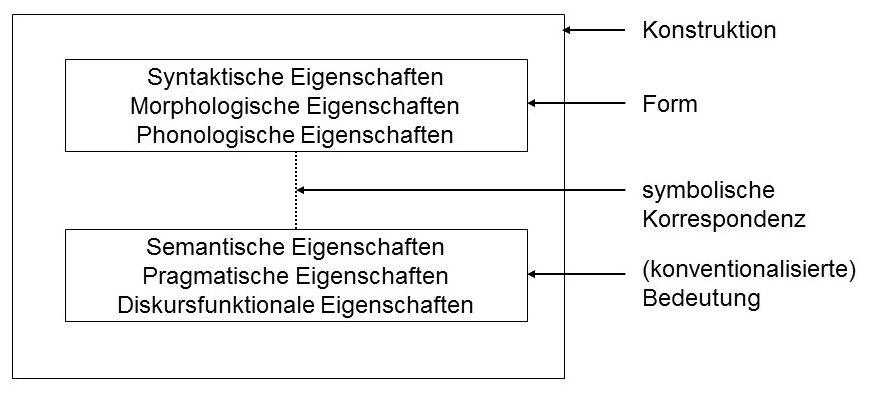
\includegraphics[width=9cm]{images/croft-construction-neu.jpg}
  \begin{tikzpicture}
  \node at (0,0) [draw,text width=7cm,align=center] (Eig1) 
    {Syntaktische Eigenschaften\\Morphologische Eigenschaften\\Phonologische Eigenschaften};
  \node [,draw, below=2\baselineskip of Eig1,text width=7cm,align=center] (Eig2) 
    {Semantische Eigenschaften\\Pragmatische Eigenschaften\\Diskursfunktionale Eigenschaften};
  \draw[dotted,thick] (Eig1) -- (Eig2) node[midway,name=midway] {};
  \node [draw,inner sep=.33cm,fit=(Eig1) (Eig2)] (konstr) {};
  \node [inner sep=0pt,right=.5cm of konstr.30] (Konstruktion) {Konstruktion};
  \path let \p1 = (Konstruktion.west), \p2  = (Eig1) in node [inner sep=0pt,anchor=west] at (\x1,\y2)
    (Form) {Form};
  \path let \p1 = (Konstruktion.west), \p2  = (midway) in node [text width=3.25cm,inner sep=0pt,anchor=west] at (\x1,\y2)
    (Korrespondenz) {symbolische\\Korrespondenz};
  \path let \p1 = (Konstruktion.west), \p2  = (Eig2) in node [text width=3.25cm,inner sep=0pt,anchor=west] at (\x1,\y2)
    (Bedeutung) {(konventionalisierte)\\Bedeutung};
  \draw[-{Triangle[]}] (Konstruktion.west) -- (konstr.30);
  \draw[-{Triangle[]}] (Form) -- (Eig1);
  \draw[-{Triangle[]}] (Korrespondenz) -- (midway);
  \draw[-{Triangle[]}] (Bedeutung) -- (Eig2);
  \end{tikzpicture}
\caption {Symbolische Struktur einer \isi{Konstruktion}  \parencite[18]{Croft2002}\label{abb:croft-construction}}
\end{figure} 

Wenn ein Strukturmuster semantische oder formale Eigenschaften besitzt, die nicht"=kom"-po"-sitionell \is{Kompositionalität} zustande kommen, diese also zusätzlich erlernt werden\linebreak müssen, liegt eine Konstruk"-tion \is{Konstruktion} vor \parencite[4]{Goldberg1995}. Ebenso, wenn ein sprachliches Muster besonders frequent gebraucht wird und sich dadurch eine mentale Repräsentation einschleift bzw. \object{entrenched} wird \parencite[93]{Goldberg2006}.\footnote{In Abschnitt \ref{sec:entrenchment} werden die für den \isi{Definitartikel} relevanten Prinzipien des \object{Entrenchment} ausführlich diskutiert.}
Konstruktionen können als primär grammatisch eingeordnet werden, wie es z.B. bei Hilfsverbkonstruktionen (etwa beim \object{going-to}-Futur) der Fall ist; sie führen dann relationale Funktionen aus und sind nicht-referentiell. Oder sie sind lexikalisch, wenn sie von referentieller und beschreibender Art sind \parencite[wie das Vollverb \object{gehen}, vgl.][58]{Traugott2015}. 

%\subsubsection{Lexikon-Grammatik-Kontinuum}

Grammatik und Lexikon einer Sprache sind keine autonomen Bereiche, sondern bilden ein Kontinuum. Dies ist die zweite wichtige Annahme, die sich aus dem oben beschriebenen  Konstruktionskonzept \is{Konstruktion} ergibt.\footnote{Argumente gegen die strikte Trennung von Grammatik und Lexikon liefern zahlreiche Studien, etwa \textcite{Goldberg2006}.} Ein \isi{Morphem} kann beispielsweise abstrakt \is{Abstraktum} (z.B. ein Plu"-ral"=Morphem) oder spezifisch (z.B. \object{Tisch}) sein. Das Gleiche gilt für größere Einheiten. So repräsentieren z.B. spezifische Idiome (\object{das Handtuch werfen}) ebenso Instanzen von schematischen Strukturen \is{Schema} wie die \is{Transitivität} Transitivkonstruktion \is{Konstruktion}   (NP\textsubscript{Akk} \object{werfen}). Gemessen an ihrer Komplexität und ihrer \isi{Schematizität} können Konstruktionen \is{Konstruktion} im Grammatik-Lexikon-Kontinuum verortet werden. Diese nicht-modulare Sicht auf Sprache hat den Vorteil, dass kategoriale Übergänge problemlos erfasst werden können, da sowohl grammatische als auch lexikalische Konstruktionen \is{Konstruktion} mit dem gleichen Analyseinstrumentarium behandelt werden. Eines der zentralen Anliegen in der Grammatikalisierungsforschung \is{Grammatikalisierung} ist es, den Übergang von freien Syntagmen zu gebundenen grammatischen Zeichen zu modellieren. Aus diesem Grund ist die \isi{Konstruktionsgrammatik} sehr gut mit der Grammatikalisierungstheorie kompatibel \parencite[zur weiterführenden Diskussion s. ][85]{Diewald2008}. 

%\subsubsection{Netzwerk von Konstruktionen}

Die Konstruktionen formen ein taxonomisch organisiertes Netzwerk, das sog. \object{\isi{Konstruktikon}} \parencite[95]{Ziem2013}, in dem formal und/oder funktional ähnliche Konstruktionen miteinander assoziiert sind \parencites()()[]{Langacker1987}[262--265]{Croft2004}[]{Bybee2010}. Das Netzwerk ist dynamisch. Abhängig vom konkreten Sprachgebrauch können  Konstruktionen \is{Konstruktion} hinzukommen oder verschwinden. \textcite[17]{Traugott2013} unterscheiden dabei zwei Typen von Konstruktionen: die \object{item}-spezifischen Mikrokonstruktionen \is{Konstruktion} und die hierarchisch übergeordneten Schemata, \is{Schema} welche ggf. Subschemata enthalten können \parencite[s. auch][]{Traugott2015}. Die im Sprachgebrauch empirisch beobachtbaren \isi{Token} werden \object{constructs} genannt.\footnote{Zur Unterscheidung von \object{constructions} und \object{constructs} vgl. u.a. \textcite[][423]{Fried2013}.} Abbildung~\ref{abb:quant-schema} zeigt die Verlinkung dieser Ebenen am Beispiel des sog. \object{quantifier schema} \parencite[aus][17]{Traugott2013}. 

\begin{figure}
% % \tikzstyle{inner} = [shape=rectangle, rounded corners, draw, align=center, text width=10em]
% % \tikzstyle{level 1} = [sibling distance=10cm]
% % \tikzstyle{level 2} = [sibling distance=5cm]
% % \begin{tikzpicture}[level distance=2cm]
% %   \node[inner] {Schema\\ (z.B.~quantifier schema)}
% %     child { 
% %     	node[inner] {Subschema\\ (z.B.~large quantity)}
% %     	  child {
% %     	  	node[inner] {Mikro\-konstruktion~1}
% %     	  	  child {node {\object{many}}}
% %     	  }
% %     	  child {
% %     	  	node[inner] {Mikrokonstruktion~2}
% %     	  	  child {node {\object{a lot of}}}
% %     	  }
% %     } 
% %     child {
% %     	node[inner] {Subschema\\ (z.B. small quantity) }
% %     	  child {
% %     	  	node[inner] {Mikrokonstruktion~3}
% %     	  	  child {node {\object{few}}}
% %     	  }
% %     	  child {
% %     	  	node[inner] {Mikrokonstruktion~4}
% %     	  	  child {node {\object{a bit of}}}
% %     	  }
% %     };
% % \end{tikzpicture}
\resizebox{\textwidth}{!}{\begin{forest}
 [Schema\\ (z.B.~quantifier schema),align=center,draw,rounded corners
    [Subschema\\ (z.B.~large quantity),align=center,draw,rounded corners
      [Mikrokonstruktion 1,draw,rounded corners [\object{any}]]
      [Mikrokonstruktion 2,draw,rounded corners [\object{a lot of}]]
    ]
    [Subschema\\ (z.B. small quantity),align=center,draw,rounded corners
      [Mikrokonstruktion 3,draw,rounded corners [\object{few}]]
      [Mikrokonstruktion 4,draw,rounded corners [\object{a bit of}]]
    ]
 ]
\end{forest}}
\caption {Hierarchische Ordnung von Konstruktionen \is{Konstruktion}  (\object{quantifier schema})\label{abb:quant-schema}}
\end{figure}
 


An der Diachronie von [\object{a lot of}\,+\,N] lässt sich illustrieren, wie eine neue Mikrokonstruktion \is{Konstruktion} ihren Platz im \isi{Konstruktikon} einnimmt: Ihre Ursprünge gehen auf das Altenglische \object{hlot} zurück, welches \is{Konkretum} konkrete, unbelebte \is{Belebtheit} Objekte denotiert und als Partitivausdruck \is{Partitiv} gebraucht wird, z.B. \object{hlot landes} \extrans{ein Stück Land} \parencite[230]{Traugott2008a}. Seit dem Mittelenglischen expandiert die Konstruktion \is{Konstruktion} auf  belebte \is{Belebtheit} Referenten (etwa \object{a lot of folks}). Als echter \object{quantifier} (wie z.B. in \object{a lot of power} \extrans{viel Macht}) kommt \object{a lot of} ab dem 19. Jh. zum Einsatz  und reiht sich in dieser nicht-partitiven Funktion neben seine Schwesterkonstruktion \object{many} ein \parencite[weiterführend s.][23--24]{Traugott2013}.


%\subsubsection{Gebrauchsbasierter Ansatz}
Durch Wiederholungen können spezifische Spracheinheiten konventionali-\linebreak siert und neue Konstruktionsknoten im Netzwerk \is{Konstruktikon}ausgebildet werden. Voraussetzung hierfür ist die menschliche Fähigkeit, Sprache mittels Erfahrung zu kategorisieren und über Abstraktionsprozesse spezifische Äußerungen mit schematischen Konstruktionen \is{Schema}\is{Konstruktion}zu assoziieren. Konstruktionen werden also gebrauchsbasiert (\object{usage-based}) und auf Grundlage allgemeiner kognitiver Kategorien erworben \parencite[u.a.][]{Langacker1987,Goldberg2006,Bybee2006,Bybee2010,Bybee2013}.

In der \isi{Konstruktionsgrammatik} wird Grammatik als dynamisches System aufgefasst, das kommunikationsbedingten Veränderungen unterliegt \parencite[35--36]{Imo2007}. Auch dieser Aspekt ist sehr gut mit der \isi{Grammatikalisierung} in Einklang zu bringen, man denke bspw. an den von  \textcite{Hopper1991} geprägten Begriff der \object{emergent grammar}. Individuelle Innovationen, die sich synchron als Sprachvariation niederschlagen \parencite{Croft2010}, haben das Potenzial, über den kognitiven Abgleich mit bestehenden Konstruktionen \object{sanktioniert} zu werden und Sprachwandel voranzutreiben \parencite[66]{Langacker1987}. 

\subsection{Konstruktionswandel und Konstruktionalisierung}\label{sec:konstruktionalisierung}\is{Konstruktionalisierung|(}

Man kann zwei Arten von konstruktionsspezifischem Sprachwandel unterscheiden: den \isi{Konstruktionswandel} und die \isi{Konstruktionalisierung} \parencite[vgl.][]{Hilpert2011,Hilpert2013,Fried2013,Traugott2013,Traugott2015,Trousdale2014}. 

Unter \isi{Konstruktionswandel} fallen diejenigen Wandelprozesse, denen Mikrokonstruktionen, d.h. lexikalisch vordefinierte Konstruktionen \is{Konstruktion} unterworfen sind. Hierzu zählen Veränderungen auf der Form- oder Inhaltsseite, z.B. der graduelle Verlust der demonstrativen Komponente beim ursprünglichen \isi{Demonstrativum}  oder die Verschmelzungstendenzen von Präposition und \isi{Definitartikel} in der Gegenwartssprache (\object{in die} > \object{inne}, \object{zu dem} > \object{zum}). \isi{Konstruktionswandel} liegt auch vor, wenn sich das Kollokationsverhalten und die Frequenz einer Mikrokonstruktion \is{Konstruktion} verändern. Im vorhergehenden Abschnitt wurde bereits angemerkt, dass die Entstehung neuer Kollokate (im Sinne von Himmelmanns \is{Expansion} \herkur{host-class expansion}, s. Abschnitt \ref{sec:parameter}) für die Herausbildung des Definitartikels konstitutiv ist. Was die Frequenz angeht, so kann man vor dem Hintergrund der zunehmenden Obligatorisierung ein Anstieg im Gebrauch von \object{dër} erwarten. 

\isi{Konstruktionswandel} subsumiert im Vergleich zur \isi{Grammatikalisierung} eine breitere Palette an Wandelphänomenen: Erstens betrifft das Konzept nicht nur Konstruktionen, die sich in Richtung des grammatischen Pols einer Sprache wandeln. Auch Lexikalisierungsprozesse, \is{Lexikalisierung} die den lexikalischen Wortschatz bereichern, z.B. in Form von Univerbierungen (\object{Tageslicht}) oder idiomatischen Wendungen (\object{ins Gras beißen}), zählen zum \isi{Konstruktionswandel} \parencite[64]{Hilpert2011}, da sich auch hier form- oder funktionsseitige Veränderungen vollziehen. Während grammatische Konstruktionen \is{Konstruktion} im Laufe der Zeit an \isi{Schematizität} und \isi{Produktivität} gewinnen, büßen lexikalische Konstruktionen beides im Laufe ihrer Entstehung ein \parencite[vgl.][164]{Traugott2013}. Zweitens berücksichtigt \isi{Konstruktionswandel} auch grammatische Wandelphänomene, die nicht den Charakteristika klassischer Grammatikalisierungen \is{Grammatikalisierung} entsprechen, etwa Wortstellungswandel \parencite[vgl.][65]{Hilpert2011}. Weil Wortstellungsmuster \is{Wortstellung} als Konstruktionen begriffen werden (nämlich als abstrakte Schemata), \is{Schema} können sie ebenfalls das Resultat von \isi{Konstruktionswandel} sein. \is{Konstruktion}

Wenn \isi{Konstruktionswandel} dazu führt, dass sich in einer Sprache ein neues konventionalisiertes Form-Funktionspaar etabliert, sprechen \textcite{Traugott2013} von \isi{Konstruktionalisierung}. Sie definieren diesen Prozess folgendermaßen:  \blockcquote[22]{Traugott2013}{Constructionalization is the creation of form\textsubscript{\textit{new}}-meaning\textsubscript{\textit{new}} (combinations of) signs. It forms new type nodes, which have new syntax or morphology and new coded meaning, in the linguistic network of a population of speakers. It is accompanied by changes in degree of schematicity,
productivity, and compositionality. The constructionalization of schemas
always results from a succession of micro-steps and is therefore gradual.
New micro-constructions may likewise be created gradually, but they may
also be instantaneous. Gradually created micro-constructions tend to be
procedural, and instantaneously tend to be
contentful.}

\noindent
Zu den \object{instantaneously created micro-constructions} zählen lexikalische Konstruktionen, denen kein \isi{Konstruktionswandel} vorausgegangen ist. \textcite[3]{Traugott2013} führen hier u.a. Konversionen oder Entlehnungen an (etwa: \object{merkeln} oder \object{Sushi}). Solche Fälle sind für die vorliegende Untersuchung nicht weiter relevant. Denn bei der Entwicklung des Definitartikels handelt es sich um einen graduell ablaufenden Prozess, der aus einer Vielzahl von \object{micro-steps} zusammengesetzt ist und die \isi{Konstruktionalisierung} des Schemas  [\object{dër}\,+\,N]  zur Folge hat. Diese Mikroschritte werden in den nächsten Abschnitten erläutert und zwar erstens vor dem Hintergrund des in der Definition genannten Parameters der \isi{Schematizität} (s. Abschnitt \ref{sec:schema}), welcher eng mit der \isi{Produktivität} und \isi{Kompositionalität} eines Sprachzeichens zusammenhängt sowie dem kognitiven Mechanismus des  \object{Entrenchment} (s.  Abschnitt \ref{sec:entrenchment}); zweitens mit Bezug auf die zentralen Mechanismen des Wandels: die \isi{Analogie} und \isi{Reanalyse} (s. Abschnitt \ref{sec:mechanismen}). 

Der entscheidende Vorzug der \isi{Konstruktionalisierung} liegt \textcite[60--62]{Traugott2015} folgend darin, dass sich die in Abschnitt \ref{sec:gram}  diskutierten Grammatikalisierungstheorien gut miteinander vereinen lassen: Während der eine Forschungszweig (mit \citealt{Lehmann1995} und \citealt{Haspelmath2004} als wichtige Vertreter) formale und\slash oder funktionale Reduktionsprozesse, wie sie typischerweise auf der Ebene der Morphosyntax und Morphonologie zu finden sind, fokussiert, betont der andere (vertreten u.a. durch \citealt{Himmelmann2004} und \citealt{Croft2006}), dass ein grammatisches Zeichen im Laufe seiner Entstehung an syntaktischer und semantisch-pragmatischer Reichweite gewinnt sowie neue Kollokationen zulässt; diese Perspektive inkludiert neben morphosyntaktischen auch diskursspezifische Wandelprozesse \parencite[vgl. den Begriff der \object{\isi{Pragmatikalisierung}} für die Entwicklung von Diskursmarkern bei][]{Auer2005}. 

Mit der konstruktionsgrammatischen Sicht \is{Konstruktionsgrammatik} spielt es keine Rolle, welcher Bereich der Grammatik von Wandel erfasst wird, so dass der Konstruktionalisierungsbegriff weit genug ist, um alle genannten Ebenen einzubeziehen. Zudem kann man aus gebrauchsbasierter Perspektive dafür argumentieren, dass formale und funktionale Reduktionsprozesse in direktem Zusammenhang zur Kontextexpansion \is{Expansion} stehen und die beiden genannten Forschungsperspektiven im Prinzip zwei Seiten derselben Medaille ausmachen: So begünstigen semantische Ausbleichungsprozesse die schrittweise Ausbreitung \is{Expansion} in neue Gebrauchskontexte \parencite[61]{Traugott2015}. Und wenn eine Konstruktion \is{Konstruktion} häufig gebraucht wird, erhöht sich die Wahrscheinlichkeit, dass sie an phonetischer Substanz und auch an \isi{Kompositionalität} einbüßt \parencite[20]{Bybee2010}.  Konstruktionsgrammatische Analysen tragen diesem vielschichtigen Wandel insofern Rechnung, als dass sie das Augenmerk sowohl auf die interne Struktur eines Sprachzeichens richten, d.h. auf die Charakteristika der einzelnen Konstituenten, als auch auf die externen Eigenschaften und damit die kontextuelle Einbindung bzw. die Restriktionen des Zeichens  \parencite[zu diesem externen/internen Kontrast s. weiterführend][]{Fried2013}.  

Dass sprachliche Elemente nicht nur isoliert betrachtet werden, sondern auch vor dem Hintergrund ihrer formalen und funktionalen Verwandtschaftsbeziehungen \is{Konstruktikon} im Konstruktionsnetzwerk, führt schließlich dazu, die Aufmerksamkeit auch auf größere systemische Zusammenhänge zu richten. In Bezug auf den \isi{Definitartikel} ist es dabei lohnenswert, die strukturellen und funktionalen Beziehungen zwischen parallel gebildeten Nominalphrasen \is{Nominalphrase (NP)} mit in die Analyse einzubeziehen. Auf Basis solcher Überlegungen deckt \textcite{Sommerer2011,Sommerer2012,Sommerer2015} bei ihren Untersuchungen zum englischen \isi{Definitartikel} auf, dass sich bereits im frühen Altenglischen durch Analogieprozesse \is{Analogie} ein abstraktes \isi{Determiniererschema} herausbildet, und zwar deswegen, weil \isi{Definitheit} schon früh mehrheitlich pränominal, z.B. in Form von Genitivattributen \is{Genitivattribut} oder Possessiva \is{Possessivum} am Nomen markiert wird. Das altenglische \isi{Demonstrativum} \object{se} wird dabei als \object{Default}-Marker für \isi{Definitheit} etabliert. In den nachfolgenden Abschnitten wird gezeigt, dass für den deutschen \isi{Definitartikel} ein ähnliches Entstehungsszenario angenommen werden darf.\is{Konstruktionalisierung|)}

\subsection{Die Herausbildung des Schemas [Definitartikel\,+\,N]}\label{sec:schema}

Wie zu Beginn von Abschnitt \ref{sec:kxg} bereits dargelegt wurde, kann man zwischen spezifischen  und abstrakten, d.h. schematischen Konstruktionstypen \is{Schema} unterscheiden. Folglich ist es möglich, Konstruktionen nach ihrem Abstraktheitsgrad einzuteilen oder anders ausgedrückt, ihnen einen bestimmten Grad an formaler und\slash oder funktionaler \isi{Schematizität} zuzuweisen. Im Gegenwartsdeutschen ist der \isi{Definitartikel} in eine teilschematische Konstruktion \is{Konstruktion}  eingebettet: [Definitartikel\,+\,N]. Der N-Slot zeichnet sich durch eine hohe Variabilität und damit \isi{Schematizität} aus, da die meisten Appellativa \is{Gattungsname} in der Standardsprache einen Artikel bei sich tragen können \parencite[zu den Ausnahmen s.][]{DAvis2013}.
Weil im Deutschen neben dem \isi{Definitartikel} noch andere pränominale Definitheitsmarker \is{Definitheit} existieren (u.a. Possessivartikel, Demonstrativartikel) \is{Possessivum}\is{Demonstrativartikel}lässt sich ein weiteres übergeordnetes \isi{Schema} ansetzen, nämlich [Determinierer\,+\,N]. Der De"-ter"-mi"-nie"-rer-Slot generalisiert dabei über alle pränominalen Elemente, die zur eindeutigen Determination des Referenten beitragen. 

%\subsubsection{Herausbildung von Schemata} 

Wie kommt es zur Entstehung solcher Schemata? Schemata \is{Schema} lassen sich definieren als \blockcquote[14]{Traugott2013}{abstractions across sets of constructions which are (unconsciously) perceived by language-users to be closely related to each other in the constructional network}. Die Voraussetzung für die Entstehung ist also, dass Sprecher auf Basis konkreter \isi{Token} Generalisierungen anstellen. Die \isi{Konstruktionalisierung} eines Schemas, die \object{\isi{Schematisierung}} \parencite[116]{Traugott2013}, nimmt ihren Ausgangspunkt damit immer auf der Ebene von Mikrokonstruktionen: Mikrokonstruktionen \is{Konstruktion} verändern sich durch den Sprachgebrauch und können dadurch zu einem neuen Konstruktionstyp abstrahiert werden. Das Resultat kann ein einzelner innovativer grammatischer Ausdruck sein (etwa eine neue Präposition, z.B. \object{auf}\textsubscript{P} \object{Grund}\textsubscript{N} \object{des} N > \object{aufgrund}\textsubscript{P} \object{des} N) oder auch eine neue grammatische Kategorie (wie das \object{going-to}-Futur). In Bezug auf den \isi{Definitartikel} bedeutet dies, dass sich die Konstruktion \is{Konstruktion}  [Demonstrativartikel\,+\,N] zur \isi{Konstruktion} [Definitartikel + N] entwickelt hat, indem das ursprünglich frei wählbare \isi{Demonstrativum} zum obligatorischen Definitheitsmarker \is{Definitheit} reanalysiert \is{Reanalyse} wurde, 
was dazu führte, dass sich \isi{Definitheit} als Nominalkategorie \is{Nominalität} etablieren konnte. Weil der ursprüngliche \isi{Demonstrativartikel} seine demonstrativen Komponenten einbüßt, gewinnt er an kombinatorischer Spannbreite. So geht aus den Daten von \textcite{Oubouzar1992,Oubouzar1997a}, die auf der bislang umfangreichsten Untersuchung zur \isi{Nominalsyntax} und zum Artikelgebrauch im Althochdeutschen basieren \parencite{Oubouzar1989}, hervor, dass sich der \isi{Definitartikel} u.a. auf Kosten des Possessivums \is{Possessivum} ausbreitet, s. Tabelle~\ref{determinierer-oubouzar}. Zu sehen sind die Häufigkeiten von Nominalgruppen (NG) mit Determinativum \object{dër} im Vergleich zu Nominalgruppen \is{Nominalphrase (NP)} mit \isi{Possessivum} in den vier größten ahd. Textdenkmälern. 

\begin{table}
\centering
\caption{Determinierer im Althochdeutschen \parencite[163]{Oubouzar1997a}}
\label{determinierer-oubouzar}
\begin{tabular} {llr@{ }rr@{ }lr}
\lsptoprule
& & \multicolumn{4}{c}{Belege für NG} & \multicolumn{1}{c}{det. NG} \\\cmidrule(lr){3-6}
{Text} & {Zeit} & \multicolumn{2}{c}{mit Det. \object{dër}} & \multicolumn{2}{c}{mit Possessivum} & {Bel. insgesamt} \\ 
\midrule                                                          
Isidor        & ca. 790     & 245  & (45,1\%)    & 132  & (24,8\%)        & 532    \\
Tatian        & ca. 830     & 582  & (44,7\%)    & 470  & (36,2\%)       & 1300   \\
Otfrid        & ca. 870     & 1318 & (53,9\%)    & 511  & (20,8\%)        & 2446   \\
Notker        & ca. 1025    & 998  & (55,1\%)    & 355  & (19,8\%)        & 1794   \\ \lspbottomrule
\end{tabular}
\end{table}

 
Die umgekehrt proportionalen Veränderungen in den Häufigkeiten hängen damit zusammen, dass der emergierende Artikel durch den allmählichen Verlust seiner demonstrativen Funktion in die Domäne des Possessivartikels \is{Possessivum} eindringt: Wurde im Isidor und Tatian die Referenz auf Körperteile noch überwiegend durch ein \isi{Possessivum} ausgedrückt (\object{in sinemo arm, sin mund, miniu ougun}), können die gleichen Bezugsverhältnisse bei später datierten Texten (Otfrid und Notker) schon häufig durch die Verwendung von \object{dër} hergestellt werden \parencite[z.B. \object{then fingar, thiu ougun}, s.][186]{Oubouzar1997a}. Der Anstieg der Typenfrequenz führt zu einer höheren \isi{Produktivität} \parencite[vgl.][]{Baayen2009,Bybee2013} und treibt dadurch die \isi{Schematizität} der \isi{Konstruktion}  nach oben. Daran wird deutlich, dass \isi{Produktivität} mit \isi{Schematizität} zusammenhängt \parencite[][]{Baayen2009}.\footnote{Zusätzlich kann auch die semantische und/oder formale Distanz einzelner Types \is{Type} zueinander die \isi{Schematizität} erhöhen, da verschiedenartige Types \is{Type} von einem äußerst abstrakten \isi{Schema} überdacht werden können \parencite[37]{Barddal2015}.} Die Entwicklung des Definitartikels \is{Definitartikel} im Deutschen ist, wie u.a. \textcite{Demske2001} zeigt, Teil einer ganzen Serie von morphosyntaktischen Umbauprozessen, die seit dem Althochdeutschen im Bereich der Nominalphrase \is{Nominalphrase (NP)} zu beobachten sind (vgl. auch Abschnitt \ref{sec:gruende}). Neben dem emergierenden \isi{Definitartikel} nehmen Possessiv- und \is{Possessivum} \isi{Demonstrativartikel} einen festen Platz links des Bezugsnomens ein. 

%\subsubsection{Die Rolle des Determiniererschemas} 

Im Rahmen einer Pilotstudie, die der vorliegenden Arbeit vorausging, wurde die \isi{Nominalsyntax} im Althochdeutschen ausschnitthaft beleuchtet \parencite{Flick2018}. Für die Analyse wurden alle Nominalphrasen \is{Nominalphrase (NP)} mit Satzgliedfunktion aus dem vierten Kapitel des ahd. Isidor nach ihrer strukturellen Beschaffenheit annotiert. \is{Annotation} Die Daten zeigen, dass mehr als die Hälfte (rund 51\%) aller NPs \is{Nominalphrase (NP)} ein pränominales und mit dem Nomen kongruierendes Element enthalten, vgl. Tabelle~\ref{NP-Flick}. Pränominale Genitivattribute, \is{Genitivattribut} die ebenfalls determinierend wirken, machen 12,2\% aller NPs \is{Nominalphrase (NP)} aus. 

\begin{table}
\centering
\caption{Strukturtypen der NPs im 4. Kapitel des ahd. Isidor \\ \parencite{Flick2018}}
\label{NP-Flick}
\begin{tabular}{lS[table-format=2.0]S[table-format=2.1]}
\lsptoprule
{Strukturtyp}                                   & {Abs.} & {\%}  \\ \midrule
Blankes Nomen                                          & 63            & 32,1         \\
\isi{Genitivattribut}\,+\,N                                    & 24            & 12,2         \\
\isi{Possessivum}\,+\,N                                          & 23            & 11,7         \\
\object{dher} (\object{selbe})\,+\,N (+ 1x schw. Adj.) (+ \isi{Genitivattribut}) & 18            & 9,2          \\
\isi{Adjektiv}\,+\,N (+ 1x \isi{Genitivattribut})                    & 15            & 7,7          \\
Zahlwort\,+\,N (+ 1x \isi{Genitivattribut})                    & 15            & 7,7          \\
\object{dher} (\object{selbe})\,+\,\isi{Adjektiv}\,+\,N (+ \isi{Genitivattribut})        & 11            & 5,6          \\
\object{dher} (\object{selbe})\,+\,Zahlwort\,+\,N (+ 1x \isi{Genitivattribut})     & 11            & 5,6          \\
N\,+\,\isi{Genitivattribut}                                    & 7             & 3,6          \\
\object{dher} (\object{selbe})\,+\,\isi{Genitivattribut}\,+\,N                     & 3             & 1,5          \\
\object{dheser} (\object{selbe})\,+\,N                                     & 3             & 1,5          \\
N\,+\,\isi{Possessivum}                                          & 2             & 1            \\
demonstr. \object{selb}\,+\,N\,+\,\isi{Genitivattribut}                   & 1             & 0,5          \\\midrule
{Gesamt}                                        & {196}  & {100} \\ \lspbottomrule
\end{tabular}
\end{table}

Es zeichnet sich also bereits in diesem frühen Schriftstück eine starke Tendenz zur pränominalen Determination des Nomens \is{Nominalsyntax} ab. Interessanterweise besteht der größte Teil an blanken Nomen (ca. 80\%) aus Unika \is{Unikum} und Eigennamen, \is{Eigenname} also Substantivtypen, die typischerweise erst spät einen \isi{Definitartikel} tragen \parencite[s. z.B.][]{Schmuck2014}. Nur ein Fünftel der undeterminierten NPs \is{Nominalphrase (NP)} gehören zu den Gattungsnamen \is{Gattungsname} (etwa \object{mund} oder \object{namo}) und damit zu den Fällen, die in einer Artikelsprache den \isi{Definitartikel} erfordern würden. Die Daten sprechen also dafür, dass sich bereits das frühe Althochdeutsche auf dem Weg befindet, ein \isi{Determiniererschema} auszubilden, in dem sich das ursprüngliche \isi{Demonstrativum} \object{dër} zur \object{Default}-Form zum Ausdruck von \isi{Definitheit} etabliert.  Ferner zeichnet sich in den Daten der \hervor{Bauplan} für die sog. \isi{Nominalklammer} ab \parencite[vgl. u.a.][ ]{Ronneberger-Sibold1994,,Ronneberger-Sibold2010a,Ronneberger-Sibold2010,Szczepaniak2011a,Flick2018}: Die einzelnen Phrasenelemente -- Artikelwörter,  Modifizierer etc. sowie der Phrasenkopf -- sorgen dafür, dass die Nominalkategorien (Kasus, \isi{Genus} und Numerus) in kooperativer \isi{Flexion} zum Ausdruck \is{Nominalklammer} gebracht werden. Für die Entwicklung des Definitartikels ist in diesem Zusammenhang vor allem die früh dokumentierte Korrelation von \object{dër} und schwach flektierten \is{Flexion} (=\,individualisierend wirkenden) Adjektiven \is{Adjektiv} von Bedeutung. Dieses \isi{Schema} hat vermutlich dazu beigetragen, dass  \object{dër} als pränominaler Determinierer obligatorisiert wurde (s. hierzu ausführlich Abschnitt~\ref{ersatz-schwach}).  In der vorliegenden Arbeit wird an die bisherige Forschung angeknüpft, indem  mit einer computergestützten Korpusuntersuchung \is{Korpuslinguistik} den NP-Strukturtypen \is{Nominalphrase (NP)} im Althochdeutschen auf den Grund gegangen wird. Ergänzend zu den Studien von \textcite{Oubouzar1989,Oubouzar1992} wird bei Übersetzungstexten auch die ahd. \isi{Wortstellung} im Vergleich zur lat. Vorlage systematisch unter die Lupe genommen (zur Aussagekraft von Differenzbelegen \is{Differenzbeleg} s. ausführlich Abschnitt \ref{sec:differenz}).   

%\subsubsection{Richtungen der Schematisierung} 

\textcite{Sommerer2012,Sommerer2015} geht in ihren Studien zur Herausbildung des englischen Definitartikels davon aus, dass die \isi{Grammatikalisierung} erst beginnen konnte, \object{nachdem} sich ein \isi{Determiniererschema} entwickelt hatte. Ihre Argumentation beruht auf einer  Korpusuntersuchung \is{Korpuslinguistik} \parencite[vgl.][197--198]{Sommerer2012}, bei der sie Nominalphrasen aus sechs altenglischen Manuskripten analysiert und nachweist, dass definite No"-mi"-nal"-phra"-sen in der großen Mehrzahl eine overte pränominale Definitheitsmarkierung \is{Definitheit} aufweisen. Weniger als 1\% der Appellativa \is{Gattungsname}  mit definiter Referenz bleiben undeterminiert \parencite[122]{Sommerer2015}. Am frequentesten ist dabei das altenglische \isi{Demonstrativum} \object{se} (der Vorläufer des gegenwärtigen englischen \object{the}), ansonsten dienen Possessivartikel \is{Possessivum} oder Genitivattribute \is{Genitivattribut} als Determinierer. Sprecherinnen und Sprecher könnten aus einem solchen empirischen Input ableiten, dass determinierte Nominalphrasen \is{Nominalphrase (NP)} im Normalfall mit einem linksstehenden Element eingeleitet werden. Sommerer zufolge erwachse daraus das Bedürfnis, ein Element als Standardwert zu verpflichten, um den Determinierer-Slot zu füllen. Das \isi{Demonstrativum} \object{se} ist deswegen prädestiniert für diese Aufgabe, weil es bereits eine hohe Ge"-brauchs"-frequenz erreicht hat -- es kommt dreimal häufiger vor als andere \isi{Determinierer} \parencite[125]{Sommerer2015}. Als Triebfeder für diese Entwicklung sieht \citeauthor{Sommerer2015} die \isi{Analogie} (vgl. hierzu auch Abschnitt \ref{sec:analogie}): Das \isi{Determiniererschema} dient dabei als kognitive Vorlage, welche auf Nomen übertragen wird, die bis dato nicht oder nur selten determiniert wurden \parencite[125]{Sommerer2015}. 

Dass ein abstrakteres \isi{Schema} als treibende Kraft hinter Wandelprozessen auf spezifischeren Ebenen steht, ist sicherlich nachvollziehbar. 
Denn im Prinzip handelt es sich dabei um nichts anderes als -- grammatikalisierungstheoretisch gesprochen -- die graduelle Eingliederung eines Sprachzeichens in ein bestehendes Paradigma und damit um einen typischen Subprozess von Grammatikalisierungen. Nach Sommerer entwickelte sich das ursprüngliche \isi{Demonstrativum} allerdings nur deswegen zum Definitartikel, weil sich zuvor überhaupt erst ein abstraktes \isi{Determiniererschema} inklusive offenem Slot etabliert hatte: \blockcquote[205]{Sommerer2012}{The slot’s emergence triggers the grammaticalization of the demonstrative \object{se}. Subsequently, the form bleaches semantically (loses its deictic force), is reduced in form [...], becomes fixed in its position and is used increasingly often (even
in NPs with generic reference).} Gegen diese kausale Verkettung lässt sich allerdings einwenden, dass durchaus Sprachen existieren, die trotz des Vorhandenseins unterschiedlicher \isi{Determinierer} keinen Artikel ausgebildet haben, so etwa die slawischen Sprachen. Beispielsweise verfügt das Russische sowohl über Demonstrativ- \is{Demonstrativartikel} als auch Possessivartikel, \is{Possessivum} jedoch nicht über einen \isi{Definitartikel}. 
 
Folgt man \textcite[194]{Himmelmann1997}, so kann die zunehmende Gebrauchsfrequenz eines Demonstrativums \is{Demonstrativum} bereits als erste Stufe im Grammatikalisierungsprozess \is{Grammatikalisierung} betrachtet werden. Denn sie begünstigt nicht nur die Stellungsfestigkeit von \isi{Demonstrativum} und Bezugsnomen, sondern ist auch ein Indikator für \is{Expansion} Kontextausweitung. Daher ist es naheliegend, dass sich erst durch den häufigen Gebrauch des ursprünglichen Demonstrativums \is{Demonstrativum} überhaupt  ein Determinierer-Slot ausbildet. Sommerer selbst räumt in einem jüngeren Beitrag ein, dass die semantische Ausbleichung des Demonstrativums \is{Demonstrativum} eine Erklärung für das hohe Vorkommen dieser Wortart in ihren Daten liefern kann und damit der ersten Phase in der \isi{Grammatikalisierung} entsprechen würde \parencite[127]{Sommerer2015}. Die damit verknüpfte Etablierung eines Determinierer-Slots markiere dann den Beginn einer zweiten Entwicklungsphase: \blockcquote[127]{Sommerer2015}{This increase usage, however, then triggers the conceptualization of the slot, which, in a second phase involving other factors, pushes the demonstrative down its grammaticalization path even further}. 
Was bei diesem Szenario jedoch noch nicht beantwortet wird, ist die Frage, warum es eigentlich zu einem Frequenzanstieg des ursprünglichen Demonstrativums \is{Demonstrativum} gekommen ist. In Kapitel \ref{forschung} werden mögliche Antworten darauf präsentiert. 

Aus der Forschungsdiskussion ist deutlich geworden, dass die Artikelentwicklung aus zwei Perspektiven beleuchtet werden muss:  Erstens ist es notwendig, die individuellen Vorkommen eines sich entwickelnden Artikels zu untersuchen und zu fragen, welche Funktionen und Kombinationsmöglichkeiten die entsprechende Form zu einem bestimmten Zeitpunkt zulässt. Zweitens müssen mögliche Analogieeffekte \is{Analogie} berücksichtigt werden, d.h. man muss formal und funktional ähnliche Konstruktionen in die Analyse einbeziehen, weil diese das Potential haben, Ausdruck eines übergeordneten Schemas \is{Schema} zu sein, welches dann in einer wechselseitigen Beziehung zu seinen spezifischen Mikrokonstruktionen \is{Konstruktion} steht. 

\subsection{Type- und Token-Entrenchment}\label{sec:entrenchment}

\begin{sloppypar}Aus der kognitiven Perspektive lassen sich die im vorhergehenden Abschnitt angesprochenen Schematisierungen \is{Schematisierung} als Fälle von \object{\isi{Entrenchment}} begreifen (s. u.a. \citealt{Langacker1987,Langacker2008,Goldberg1995,Goldberg2006,Bybee2006,Bybee2010} und \citealt{Schmid2007,Schmid2016}). 
Unter diesem erstmals von \citeauthor{Langacker1987} eingeführten Begriff versteht man die kognitive Verfestigung einer sprachlichen Einheit aufgrund erhöhter Gebrauchsfrequenz:\end{sloppypar}\blockcquote[59]{Langacker1987}{Every use of a structure has a positive impact on its degree of entrenchment, whereas extended periods of disuse have a negative impact. With repeated use, a novel structure becomes progressively entrenched, to the point of becoming a unit; moreover, units are variably entrenched depending on the frequency of their occurrence [...].} 

Für die kognitive Verfestigung (teil-)schematischer \is{Schema}\is{Konstruktion}Konstruktionen, 
etwa [\object{am} V-\object{en sein}] \parencite{Flick2016} oder \is{Transitivität} die Ditransitivkonstruktion \is{Konstruktion}  [NP\textsubscript{Nom} V NP\textsubscript{Dat} NP\textsubscript{Acc}] \parencite{Goldberg2006} ist ein hoher Gebrauch unterschiedlicher Types \is{Type} verantwortlich, da sich durch das wiederholte Parsen ein schematisches Muster als überdachende Abstraktion einschleifen kann.\footnote{Es sei an dieser Stelle angemerkt, dass Frequenzwerte natürlich nur auf der Tokenebene \is{Token} gemessen werden können, d.h. es lassen sich keine Frequenzaussagen über die abstrakte Konstruktion \is{Konstruktion}  [Definitartikel\,+\,N] machen, sondern nur über die konkret realisierten Mikrokonstruktionen, etwa \object{das Kind}.} 
Der häufige Gebrauch spezifischer \isi{Token} führt hingegen typischerweise zum \isi{Entrenchment} von lexikalisch-spe\-zi\-fisch\-en Konstruktionen. Dies ist z.B. bei Idiomen (\object{Hast du Tomaten auf den Augen?}), formelhaften Wendungen (\object{Im Namen des Vaters und des Sohnes und des heiligen Geistes}) oder auch irregulären Verbmustern der Fall. \textcite[103--104]{Ziem2013} folgend kann man hier verkürzt von Type- und Token-Entrenchment \is{Type-Entrenchment}\is{Token-Entrenchment}sprechen, vgl. Abbildung~\ref{abb:type-token-entrechment}.

\begin{figure}
% %   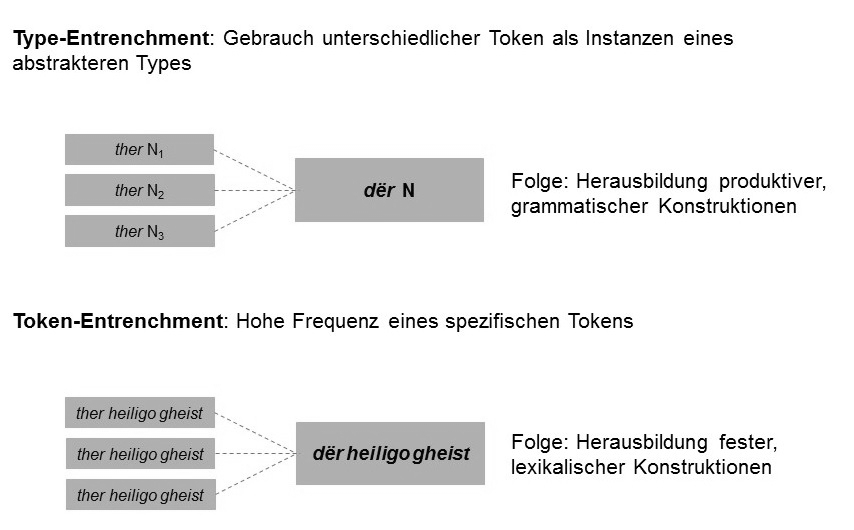
\includegraphics[width=12cm]{images/type-token-entrenchment-neu-sw.jpg}
  \fbox{\begin{minipage}{.985\textwidth}\raggedright
  \emph{\isi{Type-Entrenchment}}: Gebrauch unterschiedlicher Token als Instanzen eines abstrakten Types\\
  \begin{center}
  \begin{forest} for tree={edge={dotted,thick}}
  [\textit{dër} N,grow=west,l sep=1cm
    [\textit{ther} N\textsubscript{1}]
    [\textit{ther} N\textsubscript{2}]
    [\textit{ther} N\textsubscript{3}]
  ]
  \end{forest}\hspace{1em}\parbox[t]{.5\textwidth}{\raggedright Folge: Herausbildung produktiver, grammatischer Konstruktionen}\\
  \end{center}
  \emph{\isi{Token-Entrenchment}}: Hohe Frequenz eines spezifischen Tokens\\
  \begin{center}
  \begin{forest} for tree={edge={dotted,thick}}
  [\textit{dër heiligo gheist},grow=west,l sep=1cm
    [\textit{ther heiligo gheist}]
    [\textit{ther heiligo gheist}]
    [\textit{ther heiligo gheist}]
  ]
  \end{forest}\hspace{1em}\parbox[t]{.4\textwidth}{\raggedright Folge: Herausbildung fester, lexikalischer Konstruktionen}\\
  \end{center}
  \end{minipage}}
\caption {Type- und Token-Entrenchment} 
\label{abb:type-token-entrechment}
\end{figure} 

Indirekt kann allerdings auch \isi{Token-Entrenchment} die Ausbildung von schematischen Konstruktionen \is{Schematisierung} beeinflussen. So geht bspw. \textcite[96]{Bybee2010} davon aus, dass spezifische Konstruktionen \is{Konstruktion} Vorbild für parallel strukturierte Ausdrücke sein können und damit eine \isi{Schematisierung} ankurbeln. Sie demonstriert am Beispiel der spanischen Konstruktion \is{Konstruktion}  \object{quedarse}\,+\,\isi{Adjektiv}, dass die generellere, schematische  Konstruktion \is{Konstruktion}  über analogische Prozesse \is{Analogie} aus einem einzelnen Vorbild (dem Typ \object{quedarse sólo}) entstanden ist \parencite[72]{Bybee2010}. In Bezug auf die Herausbildung von [Definitartikel\,+\,N] kann man postulieren, dass frühe Kollokationen mit \object{dër} sich positiv auf den funktionalen Wandel von Demonstrativ- \is{Demonstrativartikel} zu \isi{Definitartikel} auswirken. So ist bspw. aus der Untersuchung von \textcite{Oubouzar1992} bekannt, dass eindeutig identifizierbare Referenten wie  z.B. \object{heilant} als Übersetzung von \object{Iesus} (im Tatian) auffallend häufig mit \object{dër} determiniert werden. Da eine zusätzliche situative \is{situativ} Verortung bzw. ein demonstrativer Verweis in diesen Fällen nicht der Grund für die Determinierung sein kann, liegen hier semantisch-definite \is{Semantische Definita}  (situationsunabhängige) Gebrauchskontexte vor, d.h. Kontexte, die ausschließlich dem \isi{Definitartikel} vorbehalten sind (s. hierzu ausführlich Abschnitt~\ref{sec:definitartikel}). Kollokationen dieser Art können damit als frühe Instanzen der Konstruktion \is{Konstruktion}  [Definitartikel + N] gewertet werden. \textcite[96]{Bybee2010} zufolge ist die immer noch vorhandene strukturelle Transparenz solcher \isi{Token} die Voraussetzung, dass Analogieprozesse \is{Analogie} stattfinden.   

Möglich ist auch, dass unterschiedliche Konstruktionen miteinander um ihren Platz im kog"-ni"-ti"-ven Netzwerk konkurrieren und so bestimmte Entrenchment-Formen \is{Entrenchment} einander blockieren. Dies ist im Deutschen -- ebenso wie in anderen germanischen Sprachen \parencite[s.][]{Himmelmann1998} -- bei adverbial \is{Adverbial} gebrauchten Präpositionalphrasen \is{Präpositionalphrase (PP)} zu beobachten. Als Teil eines Adverbials \is{Adverbial} kann ein Nomen nämlich undeterminiert bleiben, während es in Argumentpositionen ein Artikelwort braucht, vgl. \exref{ex:fuss}. Wie in Abschnitt~\ref{sec:partizipanten} noch gezeigt wird, lässt sich diese Form der Artikellosigkeit auch mit der Partizipantenrolle \is{Semantische Rolle}
 (hier: Patiens vs. Instrument) und der damit zusammenhängenden Nicht-Referentialität \is{Referentialität} erklären.  

\begin{exe}
\settowidth\jamwidth{(Objekt)}
	\ex \label{ex:fuss}
	\begin{xlist}
		\ex \label{ex:denfuss} \object{Er hält sich den Fuß.} \jambox{(Objekt)} \is{Objekt} 
		\ex \label{ex:zufuss} \object{Er läuft zu Fuß.} \jambox{(Adverbial)} \is{Adverbial}
	\end{xlist}
\end{exe}

Auch im Ahd. sind es insbesondere die in PPs eingebetteten Nomen, die sich einer Determinierung mit \object{dër} entziehen, z.B. \object{in himile} \extrans{im Himmel} oder \object{fone uuinde} \extrans{vom Winde} \parencite[84]{Oubouzar1992}; s. hierzu auch Abschnitt \ref{sec:extension}. Es scheint, als ob die Konstruktion \is{Konstruktion}  [Präp\,+\,N] so stark entrenched wurde, dass sie die emergierende Konstruktion \is{Konstruktion} [Definitartikel\,+\,N] überlagert. Phrasen ohne Artikel werden auf diese Weise syntaktisch konserviert. Je stärker der Entrenchmentgrad, \is{Entrenchment} umso resistenter ist die Konstruktion \is{Konstruktion}  gegenüber phonologischen oder morphosyntaktischen Veränderungen, denen verwandte Strukturen unterworfen sind \parencite[715]{Bybee2006}. So können sich bestimmte Types des Musters [Präp\,+\,N] bis heute zu einer eigenständigen und nicht-kompositionellen \is{Kompositionalität} \isi{Konstruktion} entwi"ckelt haben \parencite[343--344]{Himmelmann1998}. 

\isi{Entrenchment} als kognitives Prinzip bedingt die Entwicklung einer grammatischen \isi{Konstruktion}  also aus mehreren Richtungen. Es ist zum einen der Grundmechanismus für die erfolgreiche produktive Verwendung und damit der Extension eines Schemas, etwa [\object{dër}\,+\,N] oder [Präp\,+\,N]. Zum anderen kann \isi{Entrenchment} dafür sorgen, dass bestimmte \isi{Token} nicht-kompositionelle Eigenschaften \is{Kompositionalität} ausbilden. Dies ist der Fall, wenn \object{dër} in bestimmten Kollokationen bereits einen Funktionswandel von Demonstrativ- \is{Demonstrativartikel} zu \isi{Definitartikel} erfahren hat und dann in dieser Bedeutung analogisch \is{Analogie} auch mit neuen Appellativa \is{Gattungsname} gebraucht wird. 


\section{Mechanismen des Wandels}\label{sec:mechanismen}

Wenn eine neue \isi{Konstruktion}  entsteht, sind typischerweise zwei Wandelmechanismen am Werk: Vereinfacht ausgedrückt, sorgt die \isi{Analogie} für die graduelle Kontextextension, während die \isi{Reanalyse} für den Bedeutungs- und Strukturwandel zuständig ist. In der Gram"-mati"-ka"-li"-sierungs- und \is{Grammatikalisierung} daran anknüpfend  Konstruktionalisierungsforschung \is{Konstruktionalisierung} gibt es eine rege Diskussion um den Stellenwert dieser Mechanismen \parencite[vgl. u.a.][]{Haspelmath1998,Lehmann2004,Fischer2007}. In der vorliegenden Arbeit wird davon ausgegangen, dass der \isi{Definitartikel} das Resultat einer Kombination aus beidem ist --  \isi{Analogie} und \isi{Reanalyse} -- und sich die Mechanismen, wie in den nachfolgenden Abschnitten gezeigt wird, gegenseitig bedingen. Sie sind durch zwei unterschiedliche kognitive Strategien motiviert: Der \isi{Analogie} liegt das analogische Denken \is{Analogie} zugrunde, die \isi{Reanalyse} beruht auf dem syntaktischen Parsen von sprachlichem Input \parencite[38]{Traugott2013}.  


\subsection{Analogie}\label{sec:analogie}

Eine \isi{Analogie} liegt vor, wenn ein sprachlicher Ausdruck nach dem Vorbild eines bestimmten Musters (nach-)gebildet wird. So kann es z.B. innerhalb eines Flexionsparadigmas \is{Flexion} zu formalen Angleichungen kommen (=\,analogischer Ausgleich). Ein prominentes Beispiel aus der deutschen Sprachgeschichte ist die frnhd. Numerusprofilierung \parencite[1543]{Wegera2000a}, bei der die kasusmarkierenden \object{n}-Endungen der schwachen Feminina im Akkusativ, Dativ und Genitiv Singular getilgt werden und auf diese Weise Singular und Plural intraparadigmatisch formal ausdifferenzieren, s. Abbildung~\ref{abb:zunge}. Das Vorbild für die \isi{Analogie} ist der Nominativ Singular \object{zunge}. 

\begin{figure}
% %   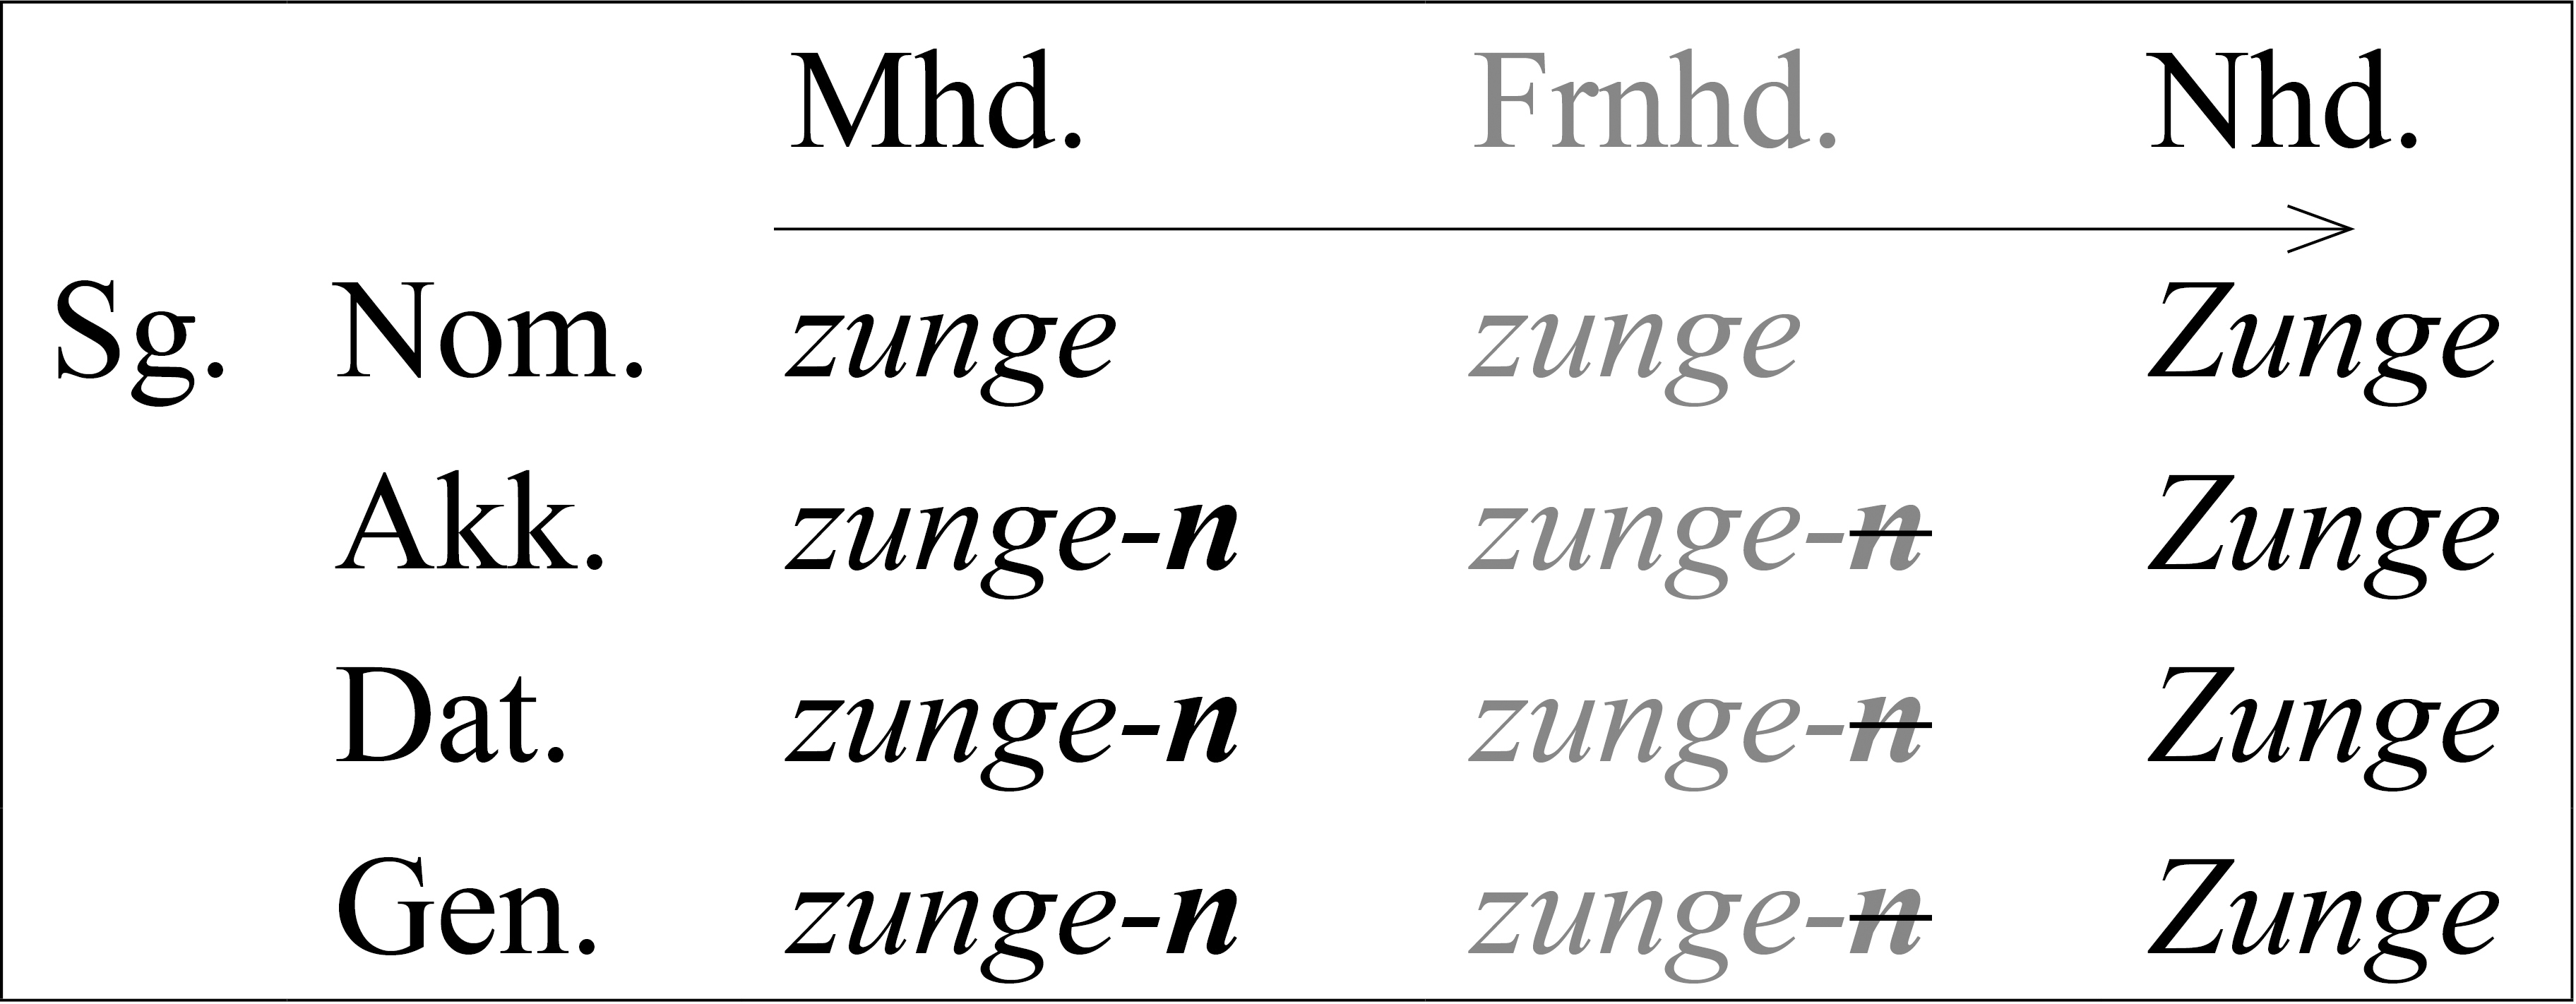
\includegraphics[width=7cm]{images/zunge.jpg}
  \begin{tabular}{ll>{\itshape}l>{\color{lsGuidelinesGray}\itshape}l>{\itshape}l}
  & & \tikzmark{Wegeramhd}\normalfont Mhd. & \upshape Frnhd. & \normalfont Nhd.\\\tablevspace
  Sg. & Nom. & zunge & zunge & Zunge\\
      & Akk. & zunge-\textbf{n} & zunge-\sout{\textbf{n}} & Zunge\\
      & Dat. & zunge-\textbf{n} & zunge-\sout{\textbf{n}} & Zunge\\
      & Gen. & zunge-\textbf{n} & zunge-\sout{\textbf{n}} & Zunge\\
  \end{tabular}
  \begin{tikzpicture}[overlay,remember picture]
  \draw[-{Triangle[]}] (pic cs:Wegeramhd)+(0,-.166) -- ++(3.8cm,-.166);
  \end{tikzpicture}
\caption {Analogischer Ausgleich bei \object{zunge}, entnommen aus \textcite[24]{Wegera2012}\label{abb:zunge}}
\end{figure} 

\textcite[160]{Lehmann2004} führt ganz ähnliche Fälle des analogischen Ausgleichs an, wenn er über die Rolle der \isi{Analogie} bei der \isi{Grammatikalisierung} spricht.\footnote{Er illustriert die \isi{Analogie} mit dem  Wandel von starker zur schwacher \isi{Flexion} bei den \is{Genus} Maskulina: mhd. \object{der hane, des hanen, die hanen} zu frnhd. \object{der Hahn, des Hahns, der Hähne}.} Seiner Meinung nach kommt die Entwicklung von Definitartikeln ganz ohne \isi{Analogie} aus, da es kein vergleichbares formales Muster gebe, das die \isi{Grammatikalisierung}  antreibe; ein analogischer Ausgleich \is{Analogie} finde also nicht statt. Lehmann sieht die Artikelentwicklung deswegen als Beweis für die Existenz von \blockcquote[161]{Lehmann2004}{pure grammaticalization without analogy}. 

Wenn man Analogien \is{Analogie} lediglich innerhalb von Flexionsparadigmen sucht, ist diese Sicht vielleicht gerechtfertigt. Analogische Prozesse \is{Analogie} reichen allerdings weit über die intraparadigmatischen Grenzen hinaus: Aus gebrauchsbasierter Sicht gleichen Sprecherinnen und Sprecher den Input, den sie bekommen, unentwegt mit bestehenden Konstruktionen \is{Konstruktion} in ihrem mentalen Netzwerk ab. Auf diese Weise kann ein existierendes Schema z.B. neue Mitglieder akquirieren. Ein prominentes Beispiel hierfür ist die Bildung von ehemals starken Verben nach dem Muster der schwachen \isi{Flexion}, z.B. mhd. \object{bellen > ball} > nhd. \object{bellen > bellte} \parencite{Bittner1985}. \isi{Analogie} ist dann gleichzusetzen mit der graduellen Ausbreitung einer \isi{Konstruktion}  auf neue Kontexte \parencite[57--58]{Bybee2010}. % Lehmann bezeichnet diesen Sprachwandel als \blockcquote[162]{Lehmann2004}{analogically-oriented grammaticalization}. 

Auch wenn kein direkt sichtbares Vorbild existiert, nach der die \isi{Konstruktion}  [Definitartikel\,+\,N] gebildet wird, so sind es dennoch analogische \is{Analogie}  Prozesse, die dem  Wandel von Demonstrativ- \is{Demonstrativartikel} zu \isi{Definitartikel} zugrunde liegen \parencite[eine ähnliche Perspektive nimmt auch Sommerer bei der Entwicklung des engl. Definitartikels ein, s.][]{Sommerer2011}. Denn sprachliche Innovationen werden von Sprecherinnen und Sprechern stets mit existierenden Knoten abgeglichen, die formal oder funktional Ähnlichkeiten aufweisen \parencite[51]{Traugott2013}. Kleinste formale und/oder funktionale Unterschiede\footnote{Langacker zufolge ist ein \blockcquote[69]{Langacker1987}{considerable amount of nonconventionality [...] tolerated (and often expected) as a normal feature of language use}.}
 können dabei Veränderungen im Konstruktionsnetzwerk bewirken:  \blockcquote[324]{Fischer2007} {The perception of similarity, or perhaps better the inability to see a difference […] between two linguistic signs or between two referents, may cause the learner/speaker to shift such an element to another set in his processing system, a set that is functionally or formally close.} Jeder innovative Gebrauch von [\object{dër}\,+\,N] veranlasst den Adressaten also, einen Abgleich mit bekannten und ähnlichen \object{chunks} \parencite[60]{Bybee2010} im mentalen Netzwerk vorzunehmen und ggf. die Verbindungen neu zu justieren. Wenn \object{dër} wiederholt in Kontexten gebraucht wird, die nicht dem prototypischen Arbeitsbereich von Demonstrativa \is{Demonstrativum} entsprechen, kann dies langfristig das Verhältnis von Form und Funktion verändern und zur Ausbildung eines neuen Schemas (vgl. Abschnitt \ref{sec:schema}) führen, das wiederum auf neue Instanzen analogisch \is{Analogie} übertragen werden kann. Konkret heißt dies, dass die demonstrative Information mit wiederholtem Gebrauch nach und nach in den Hintergrund rückt und \object{dër} als bloßer Definitheitsmarker \is{Definitheit} reanalysiert \is{Reanalyse} wird.

\subsection{Reanalyse}\label{sec:reanalyse}

Unter \isi{Reanalyse} versteht man die Um- oder Neuinterpretation\footnote{Zur Diskussion um den Vorschlag einer terminologischen Neuetikettierung von \isi{Reanalyse} zu \object{Neoanalyse} s.  \textcite[36]{Traugott2013}.} einer sprachlichen Struktur. In dieser recht weiten Definition wurde der Begriff in den vorherigen Abschnitten bereits genutzt. Vertreter eines engeren Reanalysekonzepts \is{Reanalyse} wie bspw. \textcite[215]{Heine1991} gehen davon aus, dass mit der Uminterpretation immer eine Neudefinition der Konstituentengrenzen einhergeht: \blockcquote[216]{Heine1991}{[...] we confine ourselves to what [...] is called constituent-internal reanalysis, the specific form of the more general process of reanalysis, which has the effect of redefining constituent boundaries}. Bei der \isi{Grammatikalisierung} des Definitartikels sei vor diesem Hintergrund keine \isi{Reanalyse}  beteiligt, da sowohl dem Demonstrativ- \is{Demonstrativartikel} wie dem \isi{Definitartikel} gleichermaßen der Kopfstatus in der Phrase zukäme und sich syntaktisch nichts veränderte \parencite[219]{Heine1991}. Auch in der generativen Grammatik wird die \isi{Reanalyse} als Wandelmechanismus begriffen, der die hierarchischen Verhältnisse im Satz bzw. in der Phrase beeinflusst: Das \isi{Demonstrativum}, welches ursprünglich die \object{Spec-Position} einnimmt, wird im Zuge der \isi{Grammatikalisierung} zum Kopf der NP \is{Nominalphrase (NP)} bzw. DP erhoben. Daher betrachten Vertreterinnen dieser Theorie die Herausbildung des Definitartikels als eindeutigen Fall einer syntaktischen \isi{Reanalyse} \parencite[vgl. bspw.][]{Philippi1997,vanGelderen2007}.\footnote{Zur Frage, ob das Artikelwort oder das Nomen den Kopf der Phrase bildet, s. ausführlich \textcite[145--146]{Himmelmann1997}.}

In der vorliegenden Arbeit wird \isi{Reanalyse} als kategorialer Wandel von De"-mon"-strativ- zu \isi{Definitartikel} aufgefasst, der weitere Grammatikalisierungsprozesse \is{Grammatikalisierung} (etwa die Obligatorisierung des Artikelwortes) nach sich zieht. Die \isi{Reanalyse} ist ein Prozess, der formseitig zunächst unsichtbar bleibt \parencite[58]{Langacker1977}. Erst durch die analogische \is{Analogie} Ausweitung der neuen Struktur auf neue Kontexte werden kategoriale Verschiebungen sichtbar. \textcite[50]{Hopper2006} illustrieren dies an einem Beispiel aus der Lexik: Erst die Substitution von \object{ham} durch \object{cheese} legt offen, dass das Lexem \object{hamburger} eine neue Lesart erhalten hat \parencite[urspr. \extrans{Hamburg(er) Steak}][389]{Kluge2011}. Ein aktuelles Beispiel für eine \isi{Reanalyse} auf Mehrwortebene ist die Entstehung des Rezipientenpassivs, bei dem ein adjektivisches Partizip \is{Adjektiv} verbal gedeutet wird, wie in \object{Ich bekomme den Kaffee geröstet} \parencite[152--153]{Szczepaniak2011a}.
 %oder \object{Sie hat die Daten annotiert}
Die Voraussetzung für die \isi{Reanalyse} sind also sprachliche Bausteine, die in bestimmten Kontexten ambig sind. Kategoriale \hervor{Zwitter} wie Partizipien oder Infinitive \parencite[vgl. die \isi{Reanalyse} des \object{am}-Progressivs: Aus einem nominalen wird ein verbaler Infinitiv, s.][]{Flick2013} sind prädestiniert dafür, Ambiguitäten auszulösen. 

Im Vergleich dazu verläuft die \isi{Reanalyse} des Definitartikels anders, da hier in der Spenderkonstruktion \is{Konstruktion} zunächst keine Mehrdeutigkeit angelegt ist: Am Anfang steht \hervor{nur} ein adnominales Demonstrativum. Es gibt keinen Kontext, in dem eine andere Wortart oder eine andere syntaktische Analyse möglich wäre. Um eine \isi{Reanalyse} einzuleiten, muss das \isi{Demonstrativum} in ungewöhnlichen Kontexten zum Einsatz kommen und der neue Gebrauch muss eine alternative Lesart zulassen. Wie in Abschnitt \ref{sec:kata} noch ausführlich dargelegt wird, kann man davon ausgehen, dass die Innovation, die die Entwicklung des Definitartikels ins Rollen brachte, darin bestand, dass das \isi{Demonstrativum} \object{dër} gebraucht wurde, um wichtige Referenten im Diskurs zu exponieren. Immer mehr Sprecherinnen und Sprecher imitieren diese neue diskurs"-strukturierende Maßnahme, was zur allmählichen Routinisierung und Abschwächung der Hervorhebungsfunktion führt. Die Struktur [\object{dër}\,+\,N] etabliert sich auf dem Weg dorthin als neues Schema: Aus einem fakultativ gebrauchten \isi{Demonstrativum} wird ein obligatorisch zu setzender Definitartikel. Die \isi{Reanalyse} läuft hierbei in vielen kleinen Mikroschritten ab, indem Sprecherinnen und Sprecher den sprachlichen Input immer wieder mit bestehenden Konstruktionen abgleichen und diese anpassen, was langfristig einen graduellen Wandel auf Systemebene zur Folge hat.\footnote{Zur Diskussion, inwiefern \isi{Reanalyse} abrupt oder graduell verläuft s. die Übersicht in \textcite[75]{Traugott2013}. In Bezug auf die Entwicklung des Definitartikels plädiert insbesondere \textcite{Schlachter2015} für eine abrupte \isi{Reanalyse}.} 
Dadurch wird mit jedem neuen und etwas unüblicheren Gebrauch die ursprüngliche Bedeutung von [\object{dër}\,+\,N] sozusagen überschrieben: Aus einer Demonstrativkonstruktion \is{Konstruktion}  entwickelt sich eine Definitartikelkonstruktion.

  
\section{Zusammenfassung}

Der deutsche \isi{Definitartikel} hat sich aus dem adnominal gebrauchten \isi{Demonstrativum} \object{dër} herausgebildet. Diese Entwicklung entspricht den frühen Stufen der von \textcite{Greenberg1978} und \textcite{Lehmann2015} beschriebenen, universellen Grammatikalisierungspfade \is{Grammatikalisierungspfad} für Definitartikel, welche von \textcite{Schmuck2014} für das Althochdeutsche konkretisiert wurden. Die vorliegende Arbeit setzt sich zum Ziel, diesen Pfad mithilfe einer Korpusuntersuchung \is{Korpuslinguistik} nachzuzeichnen und, wenn notwendig, neu zu modellieren. Die Entwicklung  des Definitartikels ist einerseits ein Musterbeispiel für \isi{Grammatikalisierung}, da die für diesen Sprachwandeltyp typischen Prozesse (u.a. Obligatorisierung, semantische und formale Reduktion)  durchlaufen werden. Dass am Anfang des Wandels kein lexikalisches \isi{Morphem} steht, wird in der Forschung hingegen als Besonderheit hervorgehoben. Das \isi{Demonstrativum} leistet jedoch funktional viel mehr als andere grammatische Morpheme \is{Morphem} (etwa Präpositionen). Deswegen verwundert es nicht, dass es als Quelle für Grammatikalisierungen \is{Grammatikalisierung} fungiert; in Abschnitt \ref{sec:kata} wird auf diesen Aspekt noch ausführlich eingegangen. Die Erkenntnisse aus der \isi{Grammatikalisierung} sind mit einer konstruktionsgrammatischen \is{Konstruktionsgrammatik} und gebrauchsbasierten Sprachauffassung gut vereinbar. Vor diesem Hintergrund kann die Entwicklung des Definitartikels als \isi{Konstruktionalisierung} betrachtet werden: Hierbei entsteht aus [Demonstrativartikel\,+\,N] die Konstruktion \is{Konstruktion}  [Definitartikel + N] mit der Bedeutung, Referenten als eindeutig identifizierbar zu kennzeichnen. Gleichzeitig wandeln sich die Relationen im NP-Netzwerk. Durch Entrenchment-Prozesse \is{Entrenchment} entstehen neue Knoten, darunter das abstrakte \isi{Determiniererschema}, das die Ausbreitung von \object{dër} stützt. Als zentrale Mechanismen hinter dem Wandel wurden die \isi{Analogie} und die \isi{Reanalyse} herausgearbeitet. Erstere sorgt dafür, dass [\object{dër} + N] in neuen Kontexten gebraucht wird, letztere bewirkt die neue Lesart (Definit- statt Demonstrativartikel).\is{Definitartikel}\is{Demonstrativartikel} 
